% Seminar 7: Cointegration and VECM
% Time Series Analysis -- Bachelor's programmes Economic Informatics and Economic Cybernetics, Bucharest University of Economic Studies
% GENERATED by latex/build_seminar7.py -- edit the generator, not this file.
% Student version by default; the instructor version is the *_solutions.tex wrapper.
\makeatletter\@ifundefined{ifsolutions}{\expandafter\newif\csname ifsolutions\endcsname}{}\makeatother

\newcommand{\coursename}{Time Series Analysis}
% Preambul comun TSA -- Serii de timp / Time Series Analysis (Beamer, 16:9)
% Același design ca MFM și SFM (preluat din SFM, 5 octombrie 2026). Înainte de % Preambul comun TSA -- Serii de timp / Time Series Analysis (Beamer, 16:9)
% Același design ca MFM și SFM (preluat din SFM, 5 octombrie 2026). Înainte de % Preambul comun TSA -- Serii de timp / Time Series Analysis (Beamer, 16:9)
% Același design ca MFM și SFM (preluat din SFM, 5 octombrie 2026). Înainte de \input{../../latex/preamble} se definește
%   \newcommand{\coursename}{Time Series Analysis}      (EN)
%   \newcommand{\coursename}{Serii de timp}       (RO)  și  \def\tsalang{ro}
% Fișierele .tex se află în EN/Courses, EN/Seminars, RO/Cursuri, RO/Seminarii (două niveluri sub rădăcină).
% Deck-urile sînt generate de latex/build_chapterN.py / build_seminarN.py (vezi latex/tsa_build.py).

\documentclass[9pt, aspectratio=169, t]{beamer}
\providecommand{\coursename}{Time Series Analysis}

% Ensure content fits on slides
\setbeamersize{text margin left=8mm, text margin right=8mm}
% Smaller institute font (title page)
\setbeamerfont{institute}{size=\footnotesize}

%=============================================================================
% THEME AND STYLE CONFIGURATION
%=============================================================================
\usetheme{default}
% Using default theme for clean header/footer control

% Color Palette (matching Redispatch PDF)
\definecolor{MainBlue}{RGB}{26, 58, 110}
\definecolor{AccentBlue}{RGB}{26, 58, 110}
\definecolor{IDAred}{RGB}{205, 0, 0}
\definecolor{DarkGray}{RGB}{51, 51, 51}
\definecolor{MediumGray}{RGB}{128, 128, 128}
\definecolor{LightGray}{RGB}{248, 248, 248}
\definecolor{VeryLightGray}{RGB}{235, 235, 235}
\definecolor{KeynoteGray}{RGB}{218, 218, 218}
\definecolor{SectionGray}{RGB}{120, 120, 120}
\definecolor{FooterGray}{RGB}{100, 100, 100}
\definecolor{Crimson}{RGB}{220, 53, 69}
\definecolor{Forest}{RGB}{46, 125, 50}
\definecolor{Amber}{RGB}{181, 133, 63}
\definecolor{Orange}{RGB}{230, 126, 34}
\definecolor{Purple}{RGB}{142, 68, 173}

% Gradient background (exact Keynote 315° gradient: white to RGB 218,218,218)
\setbeamertemplate{background}{%
    \begin{tikzpicture}[remember picture, overlay]
        \shade[shading=axis, shading angle=315,
        top color=white, bottom color=KeynoteGray]
        (current page.south west) rectangle (current page.north east);
    \end{tikzpicture}%
}
% Fallback solid color for compatibility
\setbeamercolor{background canvas}{bg=}

\setbeamercolor{palette primary}{bg=MainBlue, fg=white}
\setbeamercolor{palette secondary}{bg=MainBlue!85, fg=white}
\setbeamercolor{palette tertiary}{bg=MainBlue!70, fg=white}
\setbeamercolor{structure}{fg=MainBlue}
\setbeamercolor{title}{fg=IDAred}
\setbeamercolor{frametitle}{fg=IDAred, bg=}
\setbeamercolor{block title}{bg=MainBlue, fg=white}
\setbeamercolor{block body}{bg=VeryLightGray, fg=DarkGray}
\setbeamercolor{block title alerted}{bg=Crimson, fg=white}
\setbeamercolor{block body alerted}{bg=Crimson!8, fg=DarkGray}
\setbeamercolor{block title example}{bg=Forest, fg=white}
\setbeamercolor{block body example}{bg=Forest!8, fg=DarkGray}
\setbeamercolor{item}{fg=MainBlue}

% Footer colors (override Madrid theme blue)
\setbeamercolor{author in head/foot}{fg=FooterGray, bg=}
\setbeamercolor{title in head/foot}{fg=FooterGray, bg=}
\setbeamercolor{date in head/foot}{fg=FooterGray, bg=}
\setbeamercolor{section in head/foot}{fg=FooterGray, bg=}
\setbeamercolor{subsection in head/foot}{fg=FooterGray, bg=}

% Bullet styles (apply everywhere including blocks)
\setbeamertemplate{itemize item}{\color{MainBlue}$\boxdot$}
\setbeamertemplate{itemize subitem}{\color{MainBlue}$\blacktriangleright$}
\setbeamertemplate{itemize subsubitem}{\color{MainBlue}\tiny$\bullet$}
\setbeamertemplate{itemize/enumerate body begin}{\normalsize}
\setbeamertemplate{itemize/enumerate subbody begin}{\normalsize}

% Item spacing - compact style
\setlength{\leftmargini}{10pt}       % Level 1: minimal indent
\setlength{\leftmarginii}{10pt}      % Level 2: minimal additional indent
% Compact list spacing (zero extra space before/after lists in blocks)
\makeatletter
\def\@listi{\leftmargin\leftmargini \topsep 0pt \parsep 0pt \itemsep 0pt}
\def\@listii{\leftmargin\leftmarginii \topsep 0pt \parsep 0pt \itemsep 0pt}
\makeatother

\setbeamertemplate{navigation symbols}{}

%=============================================================================
% CUSTOM HEADLINE
%=============================================================================
\setbeamertemplate{headline}{%
    \vskip10pt%
    \hbox to \paperwidth{%
        \hskip0.5cm%
        {\small\color{FooterGray}\renewcommand{\hyperlink}[2]{##2}\insertsectionhead}%
        \hfill%
        \textcolor{FooterGray}{\small\insertframenumber}%
        \hskip0.5cm%
    }%
    \vskip4pt%
    {\color{FooterGray}\hrule height 0.4pt}%
}

%=============================================================================
% CUSTOM FOOTER
%=============================================================================
\usepackage{fontawesome5}

\setbeamertemplate{footline}{%
    {\color{FooterGray}\hrule height 0.4pt}%
    \vskip4pt%
    \hbox to \paperwidth{%
        \hskip0.5cm%
        \textcolor{FooterGray}{\small\coursename}%
        \hfill%
        \raisebox{-0.1em}{%
            \begin{tikzpicture}[x=0.08em, y=0.08em, line width=0.4pt]
                \draw[FooterGray] (0,3) -- (1,4) -- (2,3.5) -- (3,5) -- (4,4) -- (5,6) -- (6,5.5) -- (7,4) -- (8,5) -- (9,7) -- (10,6) -- (11,5) -- (12,6.5) -- (13,8) -- (14,7) -- (15,6) -- (16,7.5) -- (17,9) -- (18,8) -- (19,7) -- (20,8.5) -- (21,10) -- (22,9) -- (23,8) -- (24,9.5);
            \end{tikzpicture}%
        }%
        \hskip0.5cm%
    }%
    \vskip6pt%
}

%=============================================================================
% PACKAGES
%=============================================================================
\usepackage[utf8]{inputenc}
\DeclareUnicodeCharacter{03B1}{\ensuremath{\alpha}}
\usepackage[T1]{fontenc}
\usepackage{amsmath, amssymb, amsthm}
\usepackage{mathtools}
\usepackage{bm}
\usepackage{tikz}
\usetikzlibrary{arrows.meta, positioning, shapes, calc, decorations.pathreplacing, shadings}
\usepackage{booktabs}
\usepackage{multirow}
\usepackage{array}
\usepackage{graphicx}
\usepackage{animate}
\usepackage{hyperref}
\usepackage{colortbl}
\usepackage{listings}
\lstset{language=Python, basicstyle=\ttfamily\scriptsize, keywordstyle=\color{MainBlue}\bfseries,
  commentstyle=\color{Forest}, stringstyle=\color{Crimson}, breaklines=true,
  frame=none, backgroundcolor=\color{VeryLightGray}, xleftmargin=2mm}
\hypersetup{colorlinks=true, linkcolor=MainBlue, urlcolor=MainBlue}
\graphicspath{{../../logos/}{../../charts/}{../../photos/}}
\usepackage{xcolor}
\hfuzz=2pt  % Suppress tiny overfull warnings (<2pt)
\vfuzz=2pt  % Suppress tiny vertical overfull warnings (<2pt)
% \mathrm in the sans-serif family of the slides (beamer resets \mathrm to the serif family at \begin{document};
% this hook runs after beamer's, so WN, Var, RMSE, ... in formulas match the surrounding text)
% Bold vectors and matrices in the same sans-serif family: \mathbf{A} in sans bold (beamer's own \mathbf came out in
% medium weight), and the bold upright Greek capitals of \boldsymbol / \bm (\bSigma, \bPhi, \boldsymbol{\Theta}) in
% cmss bold: bm.sty fixes its "boldoperators" font when it is loaded (serif cmbx), before beamer switches the
% operators to cmss, so it is reset here.
\AtBeginDocument{%
  \SetMathAlphabet{\mathrm}{normal}{\encodingdefault}{\sfdefault}{\mddefault}{n}%
  \SetMathAlphabet{\mathrm}{bold}{\encodingdefault}{\sfdefault}{bx}{n}%
  \SetMathAlphabet{\mathbf}{normal}{\encodingdefault}{\sfdefault}{bx}{n}%
  \SetMathAlphabet{\mathbf}{bold}{\encodingdefault}{\sfdefault}{bx}{n}%
  \SetSymbolFont{boldoperators}{normal}{OT1}{cmss}{bx}{n}%
  \SetSymbolFont{boldoperators}{bold}{OT1}{cmss}{bx}{n}}

%=============================================================================
% QUANTLET COMMANDS
%   \quantlet{<displayed name>}{<url>}       (generic, compatible with the older TSA decks)
%   \tsaquantlet{Ch_05}{TSA_ch5_garch}       -> https://github.com/danpele/Time-Series-Analysis/tree/main/Quantlets/Ch_05/TSA_ch5_garch
%   \qlurl{<folder>} is defined per chapter by the generator (Quantlets/Ch_NN/<folder>)
%=============================================================================
\newcommand{\tsarepo}{https://github.com/danpele/Time-Series-Analysis}
\newcommand{\tsaqlbase}{https://github.com/danpele/Time-Series-Analysis/tree/main/Quantlets}
\newcommand{\quantlet}[2]{%
    \hfill\href{#2}{%
        \raisebox{-0.15em}{
\includegraphics[height=0.7em]{ql_logo.png}}%
        \textcolor{MainBlue}{\tiny\ #1}%
    }%
}
\newcommand{\tsaquantlet}[2]{\quantlet{\detokenize{#2}}{\tsaqlbase/#1/#2}}

%=============================================================================
% NOTEBOOKS (Google Colab)
%   \colaburl{notebooks/EN/chapter5_seminar_notebook.ipynb} -> the Colab link of a file in the TSA repo
%   \nb: the chapter notebook (each seminar deck redefines it with \renewcommand)
%=============================================================================
\newcommand{\colaburl}[1]{https://colab.research.google.com/github/danpele/Time-Series-Analysis/blob/main/#1}
\newcommand{\nb}{https://colab.research.google.com/github/danpele/Time-Series-Analysis/tree/main/notebooks/EN}
\newcommand{\nbname}{notebooks/EN}

%=============================================================================
% SLIDE HELPERS (used by the generators; the same as in MFM)
%=============================================================================
% local font size for list bodies (the preamble forces \normalsize)
\newcommand{\itemsize}[1]{\setbeamertemplate{itemize/enumerate body begin}{#1}\setbeamertemplate{itemize/enumerate subbody begin}{#1}}
\newcommand{\intitle}[1]{{\hypersetup{urlcolor=white}#1}}   % white links inside coloured title bars
\newcommand{\imgcap}[1]{{\scriptsize #1}\\[0.5mm]}          % caption under a photo
\newcommand{\imgcredit}[2]{{\tiny\color{FooterGray}\href{#1}{#2}}}   % image credit: source URL, author/licence
\newcommand{\aiprompt}[1]{{\ttfamily\color{MainBlue}#1}}     % a prompt to an AI assistant

%=============================================================================
% SEMINARS: student version by default; the instructor wrapper *_solutions.tex sets \solutionstrue
%=============================================================================
\makeatletter\@ifundefined{ifsolutions}{\expandafter\newif\csname ifsolutions\endcsname}{}\makeatother
\newcommand{\solonly}[1]{\ifsolutions #1\fi}
\newcommand{\propsub}{\ifsolutions\else\framesubtitle{\ifdefined\tsalang Rezolvarea se discută la seminar\else Solution discussed in class\fi}\fi}

%=============================================================================
% APPENDIX AND CHAPTER LINKS (latex/appendix_links.py writes the calls; it also re-declares these
% macros before \begin{document}, so the decks compile with or without this preamble block)
%=============================================================================
\providecommand{\tsaapplink}[3]{\hypertarget{#2}{}\hyperlink{#1}{\beamergotobutton{#3}}}
\providecommand{\tsaappback}[2]{\begin{tikzpicture}[remember picture,overlay]\node[anchor=south east] at ([xshift=-3mm,yshift=7mm]current page.south east){\hyperlink{#1}{\beamerreturnbutton{#2}}};\end{tikzpicture}}
\providecommand{\tsachlink}[2]{\href{#1}{#2}}
\providecommand{\tsachlinkt}[2]{\href{#1}{\usebeamercolor[fg]{frametitle}#2}}

%=============================================================================
% QUANTINAR COMMAND: link către un curs Quantinar (subiecte avansate)
%=============================================================================
\newcommand{\quantinar}[2]{%
    \href{#2}{%
        \raisebox{-0.15em}{
\includegraphics[height=0.8em]{qr_logo.png}}%
        \textcolor{MainBlue}{\scriptsize\ #1}%
    }%
}

%=============================================================================
% CUSTOM TITLE PAGE
%=============================================================================
\defbeamertemplate*{title page}{hybrid}[1][]
{
    \vspace{0.2cm}
    % Logos row - top header (with clickable links)
    \begin{center}
        \href{https://www.ase.ro}{
\includegraphics[height=1.0cm]{ase_logo.png}}\hspace{0.3cm}%
        \href{https://theida.net}{
\includegraphics[height=1.0cm]{ida_logo.png}}\hspace{0.3cm}%
        \href{https://blockchain-research-center.com}{
\includegraphics[height=1.0cm]{brc_logo.png}}\hspace{0.3cm}%
        \href{https://www.ai4efin.ase.ro}{
\includegraphics[height=1.0cm]{ai4efin_logo.png}}\hspace{0.3cm}%
        \href{https://ipe.ro/new}{
\includegraphics[height=1.0cm]{acad_logo.png}}\hspace{0.3cm}%
        \href{https://www.digital-finance-msca.com}{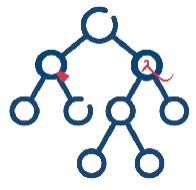
\includegraphics[height=1.0cm]{msca_logo.png}}%
    \end{center}

    \vspace{0.6cm}

    % Main title with Q logos on sides (with clickable links)
    \begin{center}
        \begin{minipage}{0.1\textwidth}
            \centering
            \href{https://quantlet.com}{
\includegraphics[height=1.1cm]{ql_logo.png}}
        \end{minipage}%
        \begin{minipage}{0.78\textwidth}
            \centering
            {\LARGE\bfseries\usebeamercolor[fg]{title}\inserttitle}

            \vspace{0.3cm}

            {\usebeamerfont{subtitle}\usebeamercolor[fg]{title}\insertsubtitle}
        \end{minipage}%
        \begin{minipage}{0.1\textwidth}
            \centering
            \href{https://quantinar.com}{
\includegraphics[height=1.1cm]{qr_logo.png}}
        \end{minipage}
    \end{center}

    \vspace{0.6cm}

    % Authors (left aligned)
    \hspace{0.5cm}{\usebeamerfont{author}\insertauthor}

    \vspace{0.3cm}

    % Institute/Affiliations (left aligned)
    \hspace{0.5cm}\begin{minipage}[t]{0.9\textwidth}
        \raggedright\small\insertinstitute
    \end{minipage}
}

%=============================================================================
% THEOREM ENVIRONMENTS
%=============================================================================
\theoremstyle{definition}
\setbeamertemplate{theorems}[numbered]
\ifdefined\tsalang
\newtheorem{defn}{Definiție}
\newtheorem{thm}{Teoremă}
\newtheorem{prop}{Propoziție}
\newtheorem{rmk}{Observație}
\else
\newtheorem{defn}{Definition}
\newtheorem{thm}{Theorem}
\newtheorem{prop}{Proposition}
\newtheorem{rmk}{Remark}
\fi

%=============================================================================
% CENTRED MINIPAGE (no extra vertical space)
%=============================================================================
\newenvironment{cminipage}[1]{%
    \par\noindent\hfill\begin{minipage}{#1}\ignorespaces
}{%
    \end{minipage}\hfill\null\par
}

%=============================================================================
% CUSTOM COMMANDS
%=============================================================================
\newcommand{\E}{\mathbb{E}}
\newcommand{\Var}{\text{Var}}
\newcommand{\Cov}{\text{Cov}}
\newcommand{\Corr}{\text{Corr}}
\newcommand{\R}{\mathbb{R}}
\newcommand{\N}{\mathbb{N}}
\newcommand{\Z}{\mathbb{Z}}
\newcommand{\B}{\mathbf{B}}
\newcommand{\imark}{\textcolor{MainBlue}{\textbullet}}
\newcommand{\RMSE}{\text{RMSE}}
\newcommand{\MAE}{\text{MAE}}
\newcommand{\MAPE}{\text{MAPE}}

% Boldface vector/matrix commands (VAR, VECM, state space; also used by the older TSA decks)
\newcommand{\bY}{\mathbf{Y}}
\newcommand{\bX}{\mathbf{X}}
\newcommand{\bA}{\mathbf{A}}
\newcommand{\bB}{\mathbf{B}}
\newcommand{\bepsilon}{\boldsymbol{\varepsilon}}
\newcommand{\bSigma}{\boldsymbol{\Sigma}}
\newcommand{\bPhi}{\boldsymbol{\Phi}}
\newcommand{\bGamma}{\boldsymbol{\Gamma}}
\newcommand{\bPi}{\boldsymbol{\Pi}}
\newcommand{\bc}{\mathbf{c}}
\newcommand{\balpha}{\boldsymbol{\alpha}}
\newcommand{\bbeta}{\boldsymbol{\beta}}
\newcommand{\bvarepsilon}{\boldsymbol{\varepsilon}}

% Legacy seminar marks (older TSA seminar decks)
\newcommand{\correct}{\textcolor{Forest}{\checkmark}}
\newcommand{\incorrect}{\textcolor{Crimson}{\texttimes}}
 se definește
%   \newcommand{\coursename}{Time Series Analysis}      (EN)
%   \newcommand{\coursename}{Serii de timp}       (RO)  și  \def\tsalang{ro}
% Fișierele .tex se află în EN/Courses, EN/Seminars, RO/Cursuri, RO/Seminarii (două niveluri sub rădăcină).
% Deck-urile sînt generate de latex/build_chapterN.py / build_seminarN.py (vezi latex/tsa_build.py).

\documentclass[9pt, aspectratio=169, t]{beamer}
\providecommand{\coursename}{Time Series Analysis}

% Ensure content fits on slides
\setbeamersize{text margin left=8mm, text margin right=8mm}
% Smaller institute font (title page)
\setbeamerfont{institute}{size=\footnotesize}

%=============================================================================
% THEME AND STYLE CONFIGURATION
%=============================================================================
\usetheme{default}
% Using default theme for clean header/footer control

% Color Palette (matching Redispatch PDF)
\definecolor{MainBlue}{RGB}{26, 58, 110}
\definecolor{AccentBlue}{RGB}{26, 58, 110}
\definecolor{IDAred}{RGB}{205, 0, 0}
\definecolor{DarkGray}{RGB}{51, 51, 51}
\definecolor{MediumGray}{RGB}{128, 128, 128}
\definecolor{LightGray}{RGB}{248, 248, 248}
\definecolor{VeryLightGray}{RGB}{235, 235, 235}
\definecolor{KeynoteGray}{RGB}{218, 218, 218}
\definecolor{SectionGray}{RGB}{120, 120, 120}
\definecolor{FooterGray}{RGB}{100, 100, 100}
\definecolor{Crimson}{RGB}{220, 53, 69}
\definecolor{Forest}{RGB}{46, 125, 50}
\definecolor{Amber}{RGB}{181, 133, 63}
\definecolor{Orange}{RGB}{230, 126, 34}
\definecolor{Purple}{RGB}{142, 68, 173}

% Gradient background (exact Keynote 315° gradient: white to RGB 218,218,218)
\setbeamertemplate{background}{%
    \begin{tikzpicture}[remember picture, overlay]
        \shade[shading=axis, shading angle=315,
        top color=white, bottom color=KeynoteGray]
        (current page.south west) rectangle (current page.north east);
    \end{tikzpicture}%
}
% Fallback solid color for compatibility
\setbeamercolor{background canvas}{bg=}

\setbeamercolor{palette primary}{bg=MainBlue, fg=white}
\setbeamercolor{palette secondary}{bg=MainBlue!85, fg=white}
\setbeamercolor{palette tertiary}{bg=MainBlue!70, fg=white}
\setbeamercolor{structure}{fg=MainBlue}
\setbeamercolor{title}{fg=IDAred}
\setbeamercolor{frametitle}{fg=IDAred, bg=}
\setbeamercolor{block title}{bg=MainBlue, fg=white}
\setbeamercolor{block body}{bg=VeryLightGray, fg=DarkGray}
\setbeamercolor{block title alerted}{bg=Crimson, fg=white}
\setbeamercolor{block body alerted}{bg=Crimson!8, fg=DarkGray}
\setbeamercolor{block title example}{bg=Forest, fg=white}
\setbeamercolor{block body example}{bg=Forest!8, fg=DarkGray}
\setbeamercolor{item}{fg=MainBlue}

% Footer colors (override Madrid theme blue)
\setbeamercolor{author in head/foot}{fg=FooterGray, bg=}
\setbeamercolor{title in head/foot}{fg=FooterGray, bg=}
\setbeamercolor{date in head/foot}{fg=FooterGray, bg=}
\setbeamercolor{section in head/foot}{fg=FooterGray, bg=}
\setbeamercolor{subsection in head/foot}{fg=FooterGray, bg=}

% Bullet styles (apply everywhere including blocks)
\setbeamertemplate{itemize item}{\color{MainBlue}$\boxdot$}
\setbeamertemplate{itemize subitem}{\color{MainBlue}$\blacktriangleright$}
\setbeamertemplate{itemize subsubitem}{\color{MainBlue}\tiny$\bullet$}
\setbeamertemplate{itemize/enumerate body begin}{\normalsize}
\setbeamertemplate{itemize/enumerate subbody begin}{\normalsize}

% Item spacing - compact style
\setlength{\leftmargini}{10pt}       % Level 1: minimal indent
\setlength{\leftmarginii}{10pt}      % Level 2: minimal additional indent
% Compact list spacing (zero extra space before/after lists in blocks)
\makeatletter
\def\@listi{\leftmargin\leftmargini \topsep 0pt \parsep 0pt \itemsep 0pt}
\def\@listii{\leftmargin\leftmarginii \topsep 0pt \parsep 0pt \itemsep 0pt}
\makeatother

\setbeamertemplate{navigation symbols}{}

%=============================================================================
% CUSTOM HEADLINE
%=============================================================================
\setbeamertemplate{headline}{%
    \vskip10pt%
    \hbox to \paperwidth{%
        \hskip0.5cm%
        {\small\color{FooterGray}\renewcommand{\hyperlink}[2]{##2}\insertsectionhead}%
        \hfill%
        \textcolor{FooterGray}{\small\insertframenumber}%
        \hskip0.5cm%
    }%
    \vskip4pt%
    {\color{FooterGray}\hrule height 0.4pt}%
}

%=============================================================================
% CUSTOM FOOTER
%=============================================================================
\usepackage{fontawesome5}

\setbeamertemplate{footline}{%
    {\color{FooterGray}\hrule height 0.4pt}%
    \vskip4pt%
    \hbox to \paperwidth{%
        \hskip0.5cm%
        \textcolor{FooterGray}{\small\coursename}%
        \hfill%
        \raisebox{-0.1em}{%
            \begin{tikzpicture}[x=0.08em, y=0.08em, line width=0.4pt]
                \draw[FooterGray] (0,3) -- (1,4) -- (2,3.5) -- (3,5) -- (4,4) -- (5,6) -- (6,5.5) -- (7,4) -- (8,5) -- (9,7) -- (10,6) -- (11,5) -- (12,6.5) -- (13,8) -- (14,7) -- (15,6) -- (16,7.5) -- (17,9) -- (18,8) -- (19,7) -- (20,8.5) -- (21,10) -- (22,9) -- (23,8) -- (24,9.5);
            \end{tikzpicture}%
        }%
        \hskip0.5cm%
    }%
    \vskip6pt%
}

%=============================================================================
% PACKAGES
%=============================================================================
\usepackage[utf8]{inputenc}
\DeclareUnicodeCharacter{03B1}{\ensuremath{\alpha}}
\usepackage[T1]{fontenc}
\usepackage{amsmath, amssymb, amsthm}
\usepackage{mathtools}
\usepackage{bm}
\usepackage{tikz}
\usetikzlibrary{arrows.meta, positioning, shapes, calc, decorations.pathreplacing, shadings}
\usepackage{booktabs}
\usepackage{multirow}
\usepackage{array}
\usepackage{graphicx}
\usepackage{animate}
\usepackage{hyperref}
\usepackage{colortbl}
\usepackage{listings}
\lstset{language=Python, basicstyle=\ttfamily\scriptsize, keywordstyle=\color{MainBlue}\bfseries,
  commentstyle=\color{Forest}, stringstyle=\color{Crimson}, breaklines=true,
  frame=none, backgroundcolor=\color{VeryLightGray}, xleftmargin=2mm}
\hypersetup{colorlinks=true, linkcolor=MainBlue, urlcolor=MainBlue}
\graphicspath{{../../logos/}{../../charts/}{../../photos/}}
\usepackage{xcolor}
\hfuzz=2pt  % Suppress tiny overfull warnings (<2pt)
\vfuzz=2pt  % Suppress tiny vertical overfull warnings (<2pt)
% \mathrm in the sans-serif family of the slides (beamer resets \mathrm to the serif family at \begin{document};
% this hook runs after beamer's, so WN, Var, RMSE, ... in formulas match the surrounding text)
% Bold vectors and matrices in the same sans-serif family: \mathbf{A} in sans bold (beamer's own \mathbf came out in
% medium weight), and the bold upright Greek capitals of \boldsymbol / \bm (\bSigma, \bPhi, \boldsymbol{\Theta}) in
% cmss bold: bm.sty fixes its "boldoperators" font when it is loaded (serif cmbx), before beamer switches the
% operators to cmss, so it is reset here.
\AtBeginDocument{%
  \SetMathAlphabet{\mathrm}{normal}{\encodingdefault}{\sfdefault}{\mddefault}{n}%
  \SetMathAlphabet{\mathrm}{bold}{\encodingdefault}{\sfdefault}{bx}{n}%
  \SetMathAlphabet{\mathbf}{normal}{\encodingdefault}{\sfdefault}{bx}{n}%
  \SetMathAlphabet{\mathbf}{bold}{\encodingdefault}{\sfdefault}{bx}{n}%
  \SetSymbolFont{boldoperators}{normal}{OT1}{cmss}{bx}{n}%
  \SetSymbolFont{boldoperators}{bold}{OT1}{cmss}{bx}{n}}

%=============================================================================
% QUANTLET COMMANDS
%   \quantlet{<displayed name>}{<url>}       (generic, compatible with the older TSA decks)
%   \tsaquantlet{Ch_05}{TSA_ch5_garch}       -> https://github.com/danpele/Time-Series-Analysis/tree/main/Quantlets/Ch_05/TSA_ch5_garch
%   \qlurl{<folder>} is defined per chapter by the generator (Quantlets/Ch_NN/<folder>)
%=============================================================================
\newcommand{\tsarepo}{https://github.com/danpele/Time-Series-Analysis}
\newcommand{\tsaqlbase}{https://github.com/danpele/Time-Series-Analysis/tree/main/Quantlets}
\newcommand{\quantlet}[2]{%
    \hfill\href{#2}{%
        \raisebox{-0.15em}{
\includegraphics[height=0.7em]{ql_logo.png}}%
        \textcolor{MainBlue}{\tiny\ #1}%
    }%
}
\newcommand{\tsaquantlet}[2]{\quantlet{\detokenize{#2}}{\tsaqlbase/#1/#2}}

%=============================================================================
% NOTEBOOKS (Google Colab)
%   \colaburl{notebooks/EN/chapter5_seminar_notebook.ipynb} -> the Colab link of a file in the TSA repo
%   \nb: the chapter notebook (each seminar deck redefines it with \renewcommand)
%=============================================================================
\newcommand{\colaburl}[1]{https://colab.research.google.com/github/danpele/Time-Series-Analysis/blob/main/#1}
\newcommand{\nb}{https://colab.research.google.com/github/danpele/Time-Series-Analysis/tree/main/notebooks/EN}
\newcommand{\nbname}{notebooks/EN}

%=============================================================================
% SLIDE HELPERS (used by the generators; the same as in MFM)
%=============================================================================
% local font size for list bodies (the preamble forces \normalsize)
\newcommand{\itemsize}[1]{\setbeamertemplate{itemize/enumerate body begin}{#1}\setbeamertemplate{itemize/enumerate subbody begin}{#1}}
\newcommand{\intitle}[1]{{\hypersetup{urlcolor=white}#1}}   % white links inside coloured title bars
\newcommand{\imgcap}[1]{{\scriptsize #1}\\[0.5mm]}          % caption under a photo
\newcommand{\imgcredit}[2]{{\tiny\color{FooterGray}\href{#1}{#2}}}   % image credit: source URL, author/licence
\newcommand{\aiprompt}[1]{{\ttfamily\color{MainBlue}#1}}     % a prompt to an AI assistant

%=============================================================================
% SEMINARS: student version by default; the instructor wrapper *_solutions.tex sets \solutionstrue
%=============================================================================
\makeatletter\@ifundefined{ifsolutions}{\expandafter\newif\csname ifsolutions\endcsname}{}\makeatother
\newcommand{\solonly}[1]{\ifsolutions #1\fi}
\newcommand{\propsub}{\ifsolutions\else\framesubtitle{\ifdefined\tsalang Rezolvarea se discută la seminar\else Solution discussed in class\fi}\fi}

%=============================================================================
% APPENDIX AND CHAPTER LINKS (latex/appendix_links.py writes the calls; it also re-declares these
% macros before \begin{document}, so the decks compile with or without this preamble block)
%=============================================================================
\providecommand{\tsaapplink}[3]{\hypertarget{#2}{}\hyperlink{#1}{\beamergotobutton{#3}}}
\providecommand{\tsaappback}[2]{\begin{tikzpicture}[remember picture,overlay]\node[anchor=south east] at ([xshift=-3mm,yshift=7mm]current page.south east){\hyperlink{#1}{\beamerreturnbutton{#2}}};\end{tikzpicture}}
\providecommand{\tsachlink}[2]{\href{#1}{#2}}
\providecommand{\tsachlinkt}[2]{\href{#1}{\usebeamercolor[fg]{frametitle}#2}}

%=============================================================================
% QUANTINAR COMMAND: link către un curs Quantinar (subiecte avansate)
%=============================================================================
\newcommand{\quantinar}[2]{%
    \href{#2}{%
        \raisebox{-0.15em}{
\includegraphics[height=0.8em]{qr_logo.png}}%
        \textcolor{MainBlue}{\scriptsize\ #1}%
    }%
}

%=============================================================================
% CUSTOM TITLE PAGE
%=============================================================================
\defbeamertemplate*{title page}{hybrid}[1][]
{
    \vspace{0.2cm}
    % Logos row - top header (with clickable links)
    \begin{center}
        \href{https://www.ase.ro}{
\includegraphics[height=1.0cm]{ase_logo.png}}\hspace{0.3cm}%
        \href{https://theida.net}{
\includegraphics[height=1.0cm]{ida_logo.png}}\hspace{0.3cm}%
        \href{https://blockchain-research-center.com}{
\includegraphics[height=1.0cm]{brc_logo.png}}\hspace{0.3cm}%
        \href{https://www.ai4efin.ase.ro}{
\includegraphics[height=1.0cm]{ai4efin_logo.png}}\hspace{0.3cm}%
        \href{https://ipe.ro/new}{
\includegraphics[height=1.0cm]{acad_logo.png}}\hspace{0.3cm}%
        \href{https://www.digital-finance-msca.com}{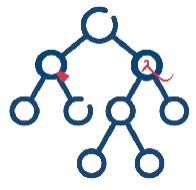
\includegraphics[height=1.0cm]{msca_logo.png}}%
    \end{center}

    \vspace{0.6cm}

    % Main title with Q logos on sides (with clickable links)
    \begin{center}
        \begin{minipage}{0.1\textwidth}
            \centering
            \href{https://quantlet.com}{
\includegraphics[height=1.1cm]{ql_logo.png}}
        \end{minipage}%
        \begin{minipage}{0.78\textwidth}
            \centering
            {\LARGE\bfseries\usebeamercolor[fg]{title}\inserttitle}

            \vspace{0.3cm}

            {\usebeamerfont{subtitle}\usebeamercolor[fg]{title}\insertsubtitle}
        \end{minipage}%
        \begin{minipage}{0.1\textwidth}
            \centering
            \href{https://quantinar.com}{
\includegraphics[height=1.1cm]{qr_logo.png}}
        \end{minipage}
    \end{center}

    \vspace{0.6cm}

    % Authors (left aligned)
    \hspace{0.5cm}{\usebeamerfont{author}\insertauthor}

    \vspace{0.3cm}

    % Institute/Affiliations (left aligned)
    \hspace{0.5cm}\begin{minipage}[t]{0.9\textwidth}
        \raggedright\small\insertinstitute
    \end{minipage}
}

%=============================================================================
% THEOREM ENVIRONMENTS
%=============================================================================
\theoremstyle{definition}
\setbeamertemplate{theorems}[numbered]
\ifdefined\tsalang
\newtheorem{defn}{Definiție}
\newtheorem{thm}{Teoremă}
\newtheorem{prop}{Propoziție}
\newtheorem{rmk}{Observație}
\else
\newtheorem{defn}{Definition}
\newtheorem{thm}{Theorem}
\newtheorem{prop}{Proposition}
\newtheorem{rmk}{Remark}
\fi

%=============================================================================
% CENTRED MINIPAGE (no extra vertical space)
%=============================================================================
\newenvironment{cminipage}[1]{%
    \par\noindent\hfill\begin{minipage}{#1}\ignorespaces
}{%
    \end{minipage}\hfill\null\par
}

%=============================================================================
% CUSTOM COMMANDS
%=============================================================================
\newcommand{\E}{\mathbb{E}}
\newcommand{\Var}{\text{Var}}
\newcommand{\Cov}{\text{Cov}}
\newcommand{\Corr}{\text{Corr}}
\newcommand{\R}{\mathbb{R}}
\newcommand{\N}{\mathbb{N}}
\newcommand{\Z}{\mathbb{Z}}
\newcommand{\B}{\mathbf{B}}
\newcommand{\imark}{\textcolor{MainBlue}{\textbullet}}
\newcommand{\RMSE}{\text{RMSE}}
\newcommand{\MAE}{\text{MAE}}
\newcommand{\MAPE}{\text{MAPE}}

% Boldface vector/matrix commands (VAR, VECM, state space; also used by the older TSA decks)
\newcommand{\bY}{\mathbf{Y}}
\newcommand{\bX}{\mathbf{X}}
\newcommand{\bA}{\mathbf{A}}
\newcommand{\bB}{\mathbf{B}}
\newcommand{\bepsilon}{\boldsymbol{\varepsilon}}
\newcommand{\bSigma}{\boldsymbol{\Sigma}}
\newcommand{\bPhi}{\boldsymbol{\Phi}}
\newcommand{\bGamma}{\boldsymbol{\Gamma}}
\newcommand{\bPi}{\boldsymbol{\Pi}}
\newcommand{\bc}{\mathbf{c}}
\newcommand{\balpha}{\boldsymbol{\alpha}}
\newcommand{\bbeta}{\boldsymbol{\beta}}
\newcommand{\bvarepsilon}{\boldsymbol{\varepsilon}}

% Legacy seminar marks (older TSA seminar decks)
\newcommand{\correct}{\textcolor{Forest}{\checkmark}}
\newcommand{\incorrect}{\textcolor{Crimson}{\texttimes}}
 se definește
%   \newcommand{\coursename}{Time Series Analysis}      (EN)
%   \newcommand{\coursename}{Serii de timp}       (RO)  și  \def\tsalang{ro}
% Fișierele .tex se află în EN/Courses, EN/Seminars, RO/Cursuri, RO/Seminarii (două niveluri sub rădăcină).
% Deck-urile sînt generate de latex/build_chapterN.py / build_seminarN.py (vezi latex/tsa_build.py).

\documentclass[9pt, aspectratio=169, t]{beamer}
\providecommand{\coursename}{Time Series Analysis}

% Ensure content fits on slides
\setbeamersize{text margin left=8mm, text margin right=8mm}
% Smaller institute font (title page)
\setbeamerfont{institute}{size=\footnotesize}

%=============================================================================
% THEME AND STYLE CONFIGURATION
%=============================================================================
\usetheme{default}
% Using default theme for clean header/footer control

% Color Palette (matching Redispatch PDF)
\definecolor{MainBlue}{RGB}{26, 58, 110}
\definecolor{AccentBlue}{RGB}{26, 58, 110}
\definecolor{IDAred}{RGB}{205, 0, 0}
\definecolor{DarkGray}{RGB}{51, 51, 51}
\definecolor{MediumGray}{RGB}{128, 128, 128}
\definecolor{LightGray}{RGB}{248, 248, 248}
\definecolor{VeryLightGray}{RGB}{235, 235, 235}
\definecolor{KeynoteGray}{RGB}{218, 218, 218}
\definecolor{SectionGray}{RGB}{120, 120, 120}
\definecolor{FooterGray}{RGB}{100, 100, 100}
\definecolor{Crimson}{RGB}{220, 53, 69}
\definecolor{Forest}{RGB}{46, 125, 50}
\definecolor{Amber}{RGB}{181, 133, 63}
\definecolor{Orange}{RGB}{230, 126, 34}
\definecolor{Purple}{RGB}{142, 68, 173}

% Gradient background (exact Keynote 315° gradient: white to RGB 218,218,218)
\setbeamertemplate{background}{%
    \begin{tikzpicture}[remember picture, overlay]
        \shade[shading=axis, shading angle=315,
        top color=white, bottom color=KeynoteGray]
        (current page.south west) rectangle (current page.north east);
    \end{tikzpicture}%
}
% Fallback solid color for compatibility
\setbeamercolor{background canvas}{bg=}

\setbeamercolor{palette primary}{bg=MainBlue, fg=white}
\setbeamercolor{palette secondary}{bg=MainBlue!85, fg=white}
\setbeamercolor{palette tertiary}{bg=MainBlue!70, fg=white}
\setbeamercolor{structure}{fg=MainBlue}
\setbeamercolor{title}{fg=IDAred}
\setbeamercolor{frametitle}{fg=IDAred, bg=}
\setbeamercolor{block title}{bg=MainBlue, fg=white}
\setbeamercolor{block body}{bg=VeryLightGray, fg=DarkGray}
\setbeamercolor{block title alerted}{bg=Crimson, fg=white}
\setbeamercolor{block body alerted}{bg=Crimson!8, fg=DarkGray}
\setbeamercolor{block title example}{bg=Forest, fg=white}
\setbeamercolor{block body example}{bg=Forest!8, fg=DarkGray}
\setbeamercolor{item}{fg=MainBlue}

% Footer colors (override Madrid theme blue)
\setbeamercolor{author in head/foot}{fg=FooterGray, bg=}
\setbeamercolor{title in head/foot}{fg=FooterGray, bg=}
\setbeamercolor{date in head/foot}{fg=FooterGray, bg=}
\setbeamercolor{section in head/foot}{fg=FooterGray, bg=}
\setbeamercolor{subsection in head/foot}{fg=FooterGray, bg=}

% Bullet styles (apply everywhere including blocks)
\setbeamertemplate{itemize item}{\color{MainBlue}$\boxdot$}
\setbeamertemplate{itemize subitem}{\color{MainBlue}$\blacktriangleright$}
\setbeamertemplate{itemize subsubitem}{\color{MainBlue}\tiny$\bullet$}
\setbeamertemplate{itemize/enumerate body begin}{\normalsize}
\setbeamertemplate{itemize/enumerate subbody begin}{\normalsize}

% Item spacing - compact style
\setlength{\leftmargini}{10pt}       % Level 1: minimal indent
\setlength{\leftmarginii}{10pt}      % Level 2: minimal additional indent
% Compact list spacing (zero extra space before/after lists in blocks)
\makeatletter
\def\@listi{\leftmargin\leftmargini \topsep 0pt \parsep 0pt \itemsep 0pt}
\def\@listii{\leftmargin\leftmarginii \topsep 0pt \parsep 0pt \itemsep 0pt}
\makeatother

\setbeamertemplate{navigation symbols}{}

%=============================================================================
% CUSTOM HEADLINE
%=============================================================================
\setbeamertemplate{headline}{%
    \vskip10pt%
    \hbox to \paperwidth{%
        \hskip0.5cm%
        {\small\color{FooterGray}\renewcommand{\hyperlink}[2]{##2}\insertsectionhead}%
        \hfill%
        \textcolor{FooterGray}{\small\insertframenumber}%
        \hskip0.5cm%
    }%
    \vskip4pt%
    {\color{FooterGray}\hrule height 0.4pt}%
}

%=============================================================================
% CUSTOM FOOTER
%=============================================================================
\usepackage{fontawesome5}

\setbeamertemplate{footline}{%
    {\color{FooterGray}\hrule height 0.4pt}%
    \vskip4pt%
    \hbox to \paperwidth{%
        \hskip0.5cm%
        \textcolor{FooterGray}{\small\coursename}%
        \hfill%
        \raisebox{-0.1em}{%
            \begin{tikzpicture}[x=0.08em, y=0.08em, line width=0.4pt]
                \draw[FooterGray] (0,3) -- (1,4) -- (2,3.5) -- (3,5) -- (4,4) -- (5,6) -- (6,5.5) -- (7,4) -- (8,5) -- (9,7) -- (10,6) -- (11,5) -- (12,6.5) -- (13,8) -- (14,7) -- (15,6) -- (16,7.5) -- (17,9) -- (18,8) -- (19,7) -- (20,8.5) -- (21,10) -- (22,9) -- (23,8) -- (24,9.5);
            \end{tikzpicture}%
        }%
        \hskip0.5cm%
    }%
    \vskip6pt%
}

%=============================================================================
% PACKAGES
%=============================================================================
\usepackage[utf8]{inputenc}
\DeclareUnicodeCharacter{03B1}{\ensuremath{\alpha}}
\usepackage[T1]{fontenc}
\usepackage{amsmath, amssymb, amsthm}
\usepackage{mathtools}
\usepackage{bm}
\usepackage{tikz}
\usetikzlibrary{arrows.meta, positioning, shapes, calc, decorations.pathreplacing, shadings}
\usepackage{booktabs}
\usepackage{multirow}
\usepackage{array}
\usepackage{graphicx}
\usepackage{animate}
\usepackage{hyperref}
\usepackage{colortbl}
\usepackage{listings}
\lstset{language=Python, basicstyle=\ttfamily\scriptsize, keywordstyle=\color{MainBlue}\bfseries,
  commentstyle=\color{Forest}, stringstyle=\color{Crimson}, breaklines=true,
  frame=none, backgroundcolor=\color{VeryLightGray}, xleftmargin=2mm}
\hypersetup{colorlinks=true, linkcolor=MainBlue, urlcolor=MainBlue}
\graphicspath{{../../logos/}{../../charts/}{../../photos/}}
\usepackage{xcolor}
\hfuzz=2pt  % Suppress tiny overfull warnings (<2pt)
\vfuzz=2pt  % Suppress tiny vertical overfull warnings (<2pt)
% \mathrm in the sans-serif family of the slides (beamer resets \mathrm to the serif family at \begin{document};
% this hook runs after beamer's, so WN, Var, RMSE, ... in formulas match the surrounding text)
% Bold vectors and matrices in the same sans-serif family: \mathbf{A} in sans bold (beamer's own \mathbf came out in
% medium weight), and the bold upright Greek capitals of \boldsymbol / \bm (\bSigma, \bPhi, \boldsymbol{\Theta}) in
% cmss bold: bm.sty fixes its "boldoperators" font when it is loaded (serif cmbx), before beamer switches the
% operators to cmss, so it is reset here.
\AtBeginDocument{%
  \SetMathAlphabet{\mathrm}{normal}{\encodingdefault}{\sfdefault}{\mddefault}{n}%
  \SetMathAlphabet{\mathrm}{bold}{\encodingdefault}{\sfdefault}{bx}{n}%
  \SetMathAlphabet{\mathbf}{normal}{\encodingdefault}{\sfdefault}{bx}{n}%
  \SetMathAlphabet{\mathbf}{bold}{\encodingdefault}{\sfdefault}{bx}{n}%
  \SetSymbolFont{boldoperators}{normal}{OT1}{cmss}{bx}{n}%
  \SetSymbolFont{boldoperators}{bold}{OT1}{cmss}{bx}{n}}

%=============================================================================
% QUANTLET COMMANDS
%   \quantlet{<displayed name>}{<url>}       (generic, compatible with the older TSA decks)
%   \tsaquantlet{Ch_05}{TSA_ch5_garch}       -> https://github.com/danpele/Time-Series-Analysis/tree/main/Quantlets/Ch_05/TSA_ch5_garch
%   \qlurl{<folder>} is defined per chapter by the generator (Quantlets/Ch_NN/<folder>)
%=============================================================================
\newcommand{\tsarepo}{https://github.com/danpele/Time-Series-Analysis}
\newcommand{\tsaqlbase}{https://github.com/danpele/Time-Series-Analysis/tree/main/Quantlets}
\newcommand{\quantlet}[2]{%
    \hfill\href{#2}{%
        \raisebox{-0.15em}{
\includegraphics[height=0.7em]{ql_logo.png}}%
        \textcolor{MainBlue}{\tiny\ #1}%
    }%
}
\newcommand{\tsaquantlet}[2]{\quantlet{\detokenize{#2}}{\tsaqlbase/#1/#2}}

%=============================================================================
% NOTEBOOKS (Google Colab)
%   \colaburl{notebooks/EN/chapter5_seminar_notebook.ipynb} -> the Colab link of a file in the TSA repo
%   \nb: the chapter notebook (each seminar deck redefines it with \renewcommand)
%=============================================================================
\newcommand{\colaburl}[1]{https://colab.research.google.com/github/danpele/Time-Series-Analysis/blob/main/#1}
\newcommand{\nb}{https://colab.research.google.com/github/danpele/Time-Series-Analysis/tree/main/notebooks/EN}
\newcommand{\nbname}{notebooks/EN}

%=============================================================================
% SLIDE HELPERS (used by the generators; the same as in MFM)
%=============================================================================
% local font size for list bodies (the preamble forces \normalsize)
\newcommand{\itemsize}[1]{\setbeamertemplate{itemize/enumerate body begin}{#1}\setbeamertemplate{itemize/enumerate subbody begin}{#1}}
\newcommand{\intitle}[1]{{\hypersetup{urlcolor=white}#1}}   % white links inside coloured title bars
\newcommand{\imgcap}[1]{{\scriptsize #1}\\[0.5mm]}          % caption under a photo
\newcommand{\imgcredit}[2]{{\tiny\color{FooterGray}\href{#1}{#2}}}   % image credit: source URL, author/licence
\newcommand{\aiprompt}[1]{{\ttfamily\color{MainBlue}#1}}     % a prompt to an AI assistant

%=============================================================================
% SEMINARS: student version by default; the instructor wrapper *_solutions.tex sets \solutionstrue
%=============================================================================
\makeatletter\@ifundefined{ifsolutions}{\expandafter\newif\csname ifsolutions\endcsname}{}\makeatother
\newcommand{\solonly}[1]{\ifsolutions #1\fi}
\newcommand{\propsub}{\ifsolutions\else\framesubtitle{\ifdefined\tsalang Rezolvarea se discută la seminar\else Solution discussed in class\fi}\fi}

%=============================================================================
% APPENDIX AND CHAPTER LINKS (latex/appendix_links.py writes the calls; it also re-declares these
% macros before \begin{document}, so the decks compile with or without this preamble block)
%=============================================================================
\providecommand{\tsaapplink}[3]{\hypertarget{#2}{}\hyperlink{#1}{\beamergotobutton{#3}}}
\providecommand{\tsaappback}[2]{\begin{tikzpicture}[remember picture,overlay]\node[anchor=south east] at ([xshift=-3mm,yshift=7mm]current page.south east){\hyperlink{#1}{\beamerreturnbutton{#2}}};\end{tikzpicture}}
\providecommand{\tsachlink}[2]{\href{#1}{#2}}
\providecommand{\tsachlinkt}[2]{\href{#1}{\usebeamercolor[fg]{frametitle}#2}}

%=============================================================================
% QUANTINAR COMMAND: link către un curs Quantinar (subiecte avansate)
%=============================================================================
\newcommand{\quantinar}[2]{%
    \href{#2}{%
        \raisebox{-0.15em}{
\includegraphics[height=0.8em]{qr_logo.png}}%
        \textcolor{MainBlue}{\scriptsize\ #1}%
    }%
}

%=============================================================================
% CUSTOM TITLE PAGE
%=============================================================================
\defbeamertemplate*{title page}{hybrid}[1][]
{
    \vspace{0.2cm}
    % Logos row - top header (with clickable links)
    \begin{center}
        \href{https://www.ase.ro}{
\includegraphics[height=1.0cm]{ase_logo.png}}\hspace{0.3cm}%
        \href{https://theida.net}{
\includegraphics[height=1.0cm]{ida_logo.png}}\hspace{0.3cm}%
        \href{https://blockchain-research-center.com}{
\includegraphics[height=1.0cm]{brc_logo.png}}\hspace{0.3cm}%
        \href{https://www.ai4efin.ase.ro}{
\includegraphics[height=1.0cm]{ai4efin_logo.png}}\hspace{0.3cm}%
        \href{https://ipe.ro/new}{
\includegraphics[height=1.0cm]{acad_logo.png}}\hspace{0.3cm}%
        \href{https://www.digital-finance-msca.com}{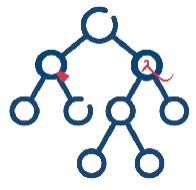
\includegraphics[height=1.0cm]{msca_logo.png}}%
    \end{center}

    \vspace{0.6cm}

    % Main title with Q logos on sides (with clickable links)
    \begin{center}
        \begin{minipage}{0.1\textwidth}
            \centering
            \href{https://quantlet.com}{
\includegraphics[height=1.1cm]{ql_logo.png}}
        \end{minipage}%
        \begin{minipage}{0.78\textwidth}
            \centering
            {\LARGE\bfseries\usebeamercolor[fg]{title}\inserttitle}

            \vspace{0.3cm}

            {\usebeamerfont{subtitle}\usebeamercolor[fg]{title}\insertsubtitle}
        \end{minipage}%
        \begin{minipage}{0.1\textwidth}
            \centering
            \href{https://quantinar.com}{
\includegraphics[height=1.1cm]{qr_logo.png}}
        \end{minipage}
    \end{center}

    \vspace{0.6cm}

    % Authors (left aligned)
    \hspace{0.5cm}{\usebeamerfont{author}\insertauthor}

    \vspace{0.3cm}

    % Institute/Affiliations (left aligned)
    \hspace{0.5cm}\begin{minipage}[t]{0.9\textwidth}
        \raggedright\small\insertinstitute
    \end{minipage}
}

%=============================================================================
% THEOREM ENVIRONMENTS
%=============================================================================
\theoremstyle{definition}
\setbeamertemplate{theorems}[numbered]
\ifdefined\tsalang
\newtheorem{defn}{Definiție}
\newtheorem{thm}{Teoremă}
\newtheorem{prop}{Propoziție}
\newtheorem{rmk}{Observație}
\else
\newtheorem{defn}{Definition}
\newtheorem{thm}{Theorem}
\newtheorem{prop}{Proposition}
\newtheorem{rmk}{Remark}
\fi

%=============================================================================
% CENTRED MINIPAGE (no extra vertical space)
%=============================================================================
\newenvironment{cminipage}[1]{%
    \par\noindent\hfill\begin{minipage}{#1}\ignorespaces
}{%
    \end{minipage}\hfill\null\par
}

%=============================================================================
% CUSTOM COMMANDS
%=============================================================================
\newcommand{\E}{\mathbb{E}}
\newcommand{\Var}{\text{Var}}
\newcommand{\Cov}{\text{Cov}}
\newcommand{\Corr}{\text{Corr}}
\newcommand{\R}{\mathbb{R}}
\newcommand{\N}{\mathbb{N}}
\newcommand{\Z}{\mathbb{Z}}
\newcommand{\B}{\mathbf{B}}
\newcommand{\imark}{\textcolor{MainBlue}{\textbullet}}
\newcommand{\RMSE}{\text{RMSE}}
\newcommand{\MAE}{\text{MAE}}
\newcommand{\MAPE}{\text{MAPE}}

% Boldface vector/matrix commands (VAR, VECM, state space; also used by the older TSA decks)
\newcommand{\bY}{\mathbf{Y}}
\newcommand{\bX}{\mathbf{X}}
\newcommand{\bA}{\mathbf{A}}
\newcommand{\bB}{\mathbf{B}}
\newcommand{\bepsilon}{\boldsymbol{\varepsilon}}
\newcommand{\bSigma}{\boldsymbol{\Sigma}}
\newcommand{\bPhi}{\boldsymbol{\Phi}}
\newcommand{\bGamma}{\boldsymbol{\Gamma}}
\newcommand{\bPi}{\boldsymbol{\Pi}}
\newcommand{\bc}{\mathbf{c}}
\newcommand{\balpha}{\boldsymbol{\alpha}}
\newcommand{\bbeta}{\boldsymbol{\beta}}
\newcommand{\bvarepsilon}{\boldsymbol{\varepsilon}}

% Legacy seminar marks (older TSA seminar decks)
\newcommand{\correct}{\textcolor{Forest}{\checkmark}}
\newcommand{\incorrect}{\textcolor{Crimson}{\texttimes}}


\newcommand{\qlurl}[1]{https://github.com/danpele/Time-Series-Analysis/tree/main/Quantlets/Ch_07/#1}
\renewcommand{\nb}{\colaburl{notebooks/EN/chapter7_seminar_notebook.ipynb}}
\renewcommand{\nbname}{chapter7\_seminar\_notebook.ipynb}
% left column: full width in the student version, narrower next to the solution
\newcommand{\taskw}{\ifsolutions 0.47\textwidth\else 0.96\textwidth\fi}
\newcommand{\solw}{\ifsolutions 0.49\textwidth\else 0pt\fi}

% Clickable citations (DOIs verified via Crossref)
\newcommand{\refHP}{\href{https://doi.org/10.1007/978-3-031-13584-2}{Huang and Petukhina (2022)}}
\newcommand{\refHamilton}{\href{https://doi.org/10.2307/j.ctv14jx6sm}{Hamilton (1994)}}
\newcommand{\refLut}{\href{https://doi.org/10.1007/978-3-540-27752-1}{Lütkepohl (2005)}}
\newcommand{\refJohBook}{\href{https://doi.org/10.1093/0198774508.001.0001}{Johansen (1995)}}
\newcommand{\refJus}{\href{https://doi.org/10.1093/oso/9780199285662.001.0001}{Juselius (2006)}}
\newcommand{\refEG}{\href{https://doi.org/10.2307/1913236}{Engle and Granger (1987)}}
\newcommand{\refGranger}{\href{https://doi.org/10.1016/0304-4076(81)90079-8}{Granger (1981)}}
\newcommand{\refGrangerN}{\href{https://doi.org/10.1257/0002828041464669}{Granger (2004)}}
\newcommand{\refGN}{\href{https://doi.org/10.1016/0304-4076(74)90034-7}{Granger and Newbold (1974)}}
\newcommand{\refMurray}{\href{https://doi.org/10.1080/00031305.1994.10476017}{Murray (1994)}}
\newcommand{\refPO}{\href{https://doi.org/10.2307/2938339}{Phillips and Ouliaris (1990)}}
\newcommand{\refMacKinnon}{\href{https://doi.org/10.1080/07350015.1994.10510005}{MacKinnon (1994)}}
\newcommand{\refMacKinnonb}{\href{https://ideas.repec.org/p/qed/wpaper/1227.html}{MacKinnon (2010)}}
\newcommand{\refSW}{\href{https://doi.org/10.1080/01621459.1988.10478707}{Stock and Watson (1988)}}
\newcommand{\refSWd}{\href{https://doi.org/10.2307/2951763}{Stock and Watson (1993)}}
\newcommand{\refDHSY}{\href{https://doi.org/10.2307/2231972}{Davidson et al.\ (1978)}}
\newcommand{\refBDM}{\href{https://doi.org/10.1111/1467-9892.00091}{Banerjee, Dolado and Mestre (1998)}}
\newcommand{\refJohA}{\href{https://doi.org/10.1016/0165-1889(88)90041-3}{Johansen (1988)}}
\newcommand{\refJohB}{\href{https://doi.org/10.2307/2938278}{Johansen (1991)}}
\newcommand{\refJJ}{\href{https://doi.org/10.1111/j.1468-0084.1990.mp52002003.x}{Johansen and Juselius (1990)}}
\newcommand{\refOL}{\href{https://doi.org/10.1111/j.1468-0084.1992.tb00013.x}{Osterwald-Lenum (1992)}}
\newcommand{\refMHM}{\href{https://doi.org/10.1002/(SICI)1099-1255(199909/10)14:5<563::AID-JAE530>3.0.CO;2-R}{MacKinnon, Haug and Michelis (1999)}}
\newcommand{\refRA}{\href{https://doi.org/10.1111/j.1467-9892.1992.tb00113.x}{Reinsel and Ahn (1992)}}
\newcommand{\refEY}{\href{https://doi.org/10.1016/0304-4076(87)90085-6}{Engle and Yoo (1987)}}
\newcommand{\refCD}{\href{https://doi.org/10.1080/07350015.1998.10524784}{Christoffersen and Diebold (1998)}}
\newcommand{\refCS}{\href{https://doi.org/10.1086/261502}{Campbell and Shiller (1987)}}
\newcommand{\refBalassa}{\href{https://doi.org/10.1086/258965}{Balassa (1964)}}
\newcommand{\refTT}{\href{https://doi.org/10.1257/0895330042632744}{Taylor and Taylor (2004)}}
\newcommand{\refGGR}{\href{https://doi.org/10.1093/rfs/hhj020}{Gatev, Goetzmann and Rouwenhorst (2006)}}
\newcommand{\refDoFaff}{\href{https://doi.org/10.2469/faj.v66.n4.1}{Do and Faff (2010)}}

\title[Time Series Analysis]{Time Series Analysis}
\subtitle{Seminar 7: Cointegration and VECM\ifsolutions\ (instructor version)\fi}
\author[D.T. Pele]{Daniel Traian PELE}
\institute{Bucharest University of Economic Studies\\
IDA Institute Digital Assets\\
Blockchain Research Center\\
AI4EFin Artificial Intelligence for Energy Finance\\
Romanian Academy, Institute for Economic Forecasting\\
MSCA Digital Finance}
\date{}

%=============================================================================
\providecommand{\tsaapplink}[3]{\hypertarget{#2}{}\hyperlink{#1}{\beamergotobutton{#3}}}  % APPLINKS-MACROS
\providecommand{\tsaappback}[2]{\begin{tikzpicture}[remember picture,overlay]\node[anchor=south east] at ([xshift=-3mm,yshift=7mm]current page.south east){\hyperlink{#1}{\beamerreturnbutton{#2}}};\end{tikzpicture}}  % APPLINKS-MACROS
\providecommand{\tsachlink}[2]{\href{#1}{#2}}  % APPLINKS-MACROS
\providecommand{\tsachlinkt}[2]{\href{#1}{\usebeamercolor[fg]{frametitle}#2}}  % APPLINKS-MACROS
\begin{document}
%=============================================================================

{
\setbeamertemplate{headline}{}
\setbeamertemplate{footline}{}
\begin{frame}[noframenumbering]
    \titlepage
\end{frame}
}
% BEGIN-ACRONYMS (generat de latex/acronyms.py; nu editati manual)
\begin{frame}{Acronyms used in this material}
\setbeamertemplate{itemize/enumerate body begin}{\tiny}
\begin{columns}[T]
\begin{column}{0.49\textwidth}
\begin{itemize}\setlength{\itemsep}{0pt}
    \item \textbf{ADF}: Augmented Dickey–Fuller (test)
    \item \textbf{AI}: Artificial Intelligence
    \item \textbf{BIC}: Bayesian Information Criterion
    \item \textbf{BNR}: Banca Națională a României (the National Bank of Romania)
    \item \textbf{BVB}: Bursa de Valori București (the Bucharest Stock Exchange)
    \item \textbf{ECM}: Error Correction Model
    \item \textbf{EODHD}: EOD Historical Data (market-data provider)
    \item \textbf{FRED}: Federal Reserve Economic Data
    \item \textbf{GDP}: Gross Domestic Product
    \item \textbf{GS1}: 1-year Treasury constant-maturity yield (FRED series code)
    \item \textbf{GS10}: 10-year Treasury constant-maturity yield (FRED series code)
    \item \textbf{HUF}: Hungarian forint (ISO 4217 code)
    \item \textbf{OLS}: Ordinary Least Squares
\end{itemize}
\end{column}
\begin{column}{0.49\textwidth}
\begin{itemize}\setlength{\itemsep}{0pt}
    \item \textbf{PLN}: Polish zloty (ISO 4217 code)
    \item \textbf{ROBOR}: Romanian Interbank Offer Rate
    \item \textbf{US}: United States
    \item \textbf{VAR}: Vector AutoRegression
    \item \textbf{VECM}: Vector Error Correction Model
\end{itemize}
\end{column}
\end{columns}
\end{frame}
% END-ACRONYMS

\begin{frame}{Today's question and route}
\itemsize{\small}
\begin{itemize}
    \item \textbf{Question}: are two or more $I(1)$ series tied by a long-run equilibrium, how fast do they return to it, and who does the adjusting?
    \begin{itemize}
        \item this seminar comes \textbf{before} Lecture 7: the section ``What you need today'' gives every definition the tasks use
    \end{itemize}
    \item Route
    \begin{itemize}
        \item Part A: Engle--Granger statistics by hand; an ECM and its half-life; a bivariate VECM; Johansen statistics; from a VAR to a VECM
        \item Part B: US interest rates; Romanian consumption and GDP; EUR/RON, EUR/HUF and EUR/PLN; ROBOR, the Romanian 10-year yield and Euribor
        \item Part C: pairs trading on two Romanian banks, and an AI answer to audit
    \end{itemize}
    \item Notebook for today: \href{\nb}{open the seminar notebook in Google Colab}; each task names its notebook section
\end{itemize}
\end{frame}

\begin{frame}{Exercise map}
\itemsize{\small}
\begin{center}
\footnotesize
\begin{tabular}{>{\raggedright\arraybackslash}p{1.1cm}>{\raggedright\arraybackslash}p{7.5cm}>{\raggedright\arraybackslash}p{1.9cm}>{\raggedright\arraybackslash}p{1.4cm}}
\toprule
\textbf{Task} & \textbf{Question} & \textbf{Type} & \textbf{Model} \\
\midrule
A1, A2 & an Engle--Granger statistic with two and with three variables & Solved, Proposed & A1 \\
A3, A4 & an ECM and a bivariate VECM: speed and half-life & Solved, Proposed & A3 \\
A5, A6 & Johansen statistics from eigenvalues; a VAR(2) written as a VECM & Solved, Proposed & A5 \\
B1, B2 & Engle--Granger and ECM: US yields; Romanian consumption and GDP & Solved, Proposed & B1 \\
B3, B4 & Johansen and VECM: three currencies; three interest rates & Solved, Proposed & B3 \\
C1, C2 & pairs trading out of sample; what is wrong in an AI answer? & Proposed & B1, B3 \\
\bottomrule
\end{tabular}
\end{center}
\begin{itemize}
    \item \textbf{[Solved]}: full solution in the slides and in the notebook, a model to follow; \textbf{[Proposed]}: you solve it, following the model
\end{itemize}
\end{frame}

\begin{frame}{Data used}
\itemsize{\small}
\begin{center}
\footnotesize
\begin{tabular}{llll}
\toprule
\textbf{Series} & \textbf{Source} & \textbf{Frequency} & \textbf{Period} \\
\midrule
US Treasury yields, 1 and 10 years & FRED (GS1, GS10) & monthly & 1960--2026 \\
Household consumption and GDP, Romania & Eurostat (namq\_10\_gdp) & quarterly, SA & 1995--2026 \\
EUR/RON, EUR/HUF, EUR/PLN & BNR reference rates & month-end & 2005--2026 \\
ROBOR 3M, Euribor 3M & Eurostat (irt\_st\_m) & monthly & 2010--2026 \\
Romanian 10-year yield & EODHD & daily, monthly mean & 2010--2026 \\
Banca Transilvania, BRD & EODHD & daily, adjusted close & 2014--2026 \\
\bottomrule
\end{tabular}
\end{center}
\begin{itemize}
    \item Levels as $100\ln$ (consumption, GDP, exchange rates, share prices); interest rates in \% per year
    \item In the notebook: \texttt{adf\_test}, \texttt{eg\_test} (Engle--Granger and Phillips--Ouliaris), \texttt{ecm\_fit}, \texttt{johansen}; no account or key is needed
\end{itemize}
\end{frame}


%=============================================================================
\section{What you need today}
%=============================================================================

\begin{frame}{What you need today (1/4): cointegration}
\itemsize{\small}
\begin{itemize}
    \item $y_t \sim I(1)$: $y_t$ has a unit root and $\Delta y_t = y_t - y_{t-1}$ is stationary (\tsachlink{https://danpele.github.io/Time-Series-Analysis/EN/Courses/chapter3_unit_roots_arima_models.pdf}{Chapter 3}; ADF test, $H_0$: unit root)
    \begin{itemize}
        \item regressing one $I(1)$ series on another, unrelated one gives a \textbf{spurious regression}: large $t$, high $R^2$
    \end{itemize}
    \item \textbf{Cointegration}: $I(1)$ series $y_{1t}, \dots, y_{nt}$ for which a combination $\beta^\top\mathbf y_t$ is stationary
    \begin{itemize}
        \item $\beta$: the cointegrating vector, normalised with one coefficient equal to 1; $u_t = \beta^\top\mathbf y_t - \mu$: the equilibrium error
        \item the series share common stochastic trends: $n$ variables, $r$ cointegrating vectors, $n - r$ common trends
    \end{itemize}
    \item Example: the 1-year and the 10-year interest rate wander, but their spread stays within a band
\end{itemize}
\end{frame}

\begin{frame}{What you need today (2/4): the Engle--Granger test}
\itemsize{\small}
\begin{itemize}
    \item \textbf{Step 1}: OLS in levels, $y_t = a + b x_t + u_t$; residuals $\hat u_t$
    \begin{itemize}
        \item \textbf{Step 2}: ADF on $\hat u_t$ without constant: $\Delta\hat u_t = \gamma\hat u_{t-1} + \sum_j\delta_j\Delta\hat u_{t-j} + e_t$, $\tau = \hat\gamma/\mathrm{SE}(\hat\gamma)$
        \item $H_0$: no cointegration ($\gamma = 0$); reject if $\tau$ is below the critical value
    \end{itemize}
    \item \textbf{Critical values} (MacKinnon, with a constant, large $T$): more negative than Dickey--Fuller, because OLS makes $\hat u_t$ look stationary
    \begin{itemize}
        \item 5\%: $-2.86$ (one series, Dickey--Fuller); $-3.34$ (2 variables); $-3.74$ (3 variables)
    \end{itemize}
    \item \textbf{Phillips--Ouliaris} $Z_t$: the same $H_0$ and critical values; no lags, a long-run variance correction
    \begin{itemize}
        \item in Python: \texttt{coint} (\texttt{statsmodels}), \texttt{phillips\_ouliaris} (\texttt{arch})
    \end{itemize}
\end{itemize}
\end{frame}

\begin{frame}{What you need today (3/4): error correction}
\itemsize{\small}
\begin{itemize}
    \item \textbf{ECM} (error correction model): $\Delta y_t = c + \gamma\,\hat u_{t-1} + \delta_0\,\Delta x_t + \dots + \varepsilon_t$, with $\hat u_{t-1} = y_{t-1} - \hat a - \hat b x_{t-1}$
    \begin{itemize}
        \item $\gamma < 0$: \textbf{speed of adjustment}, the share of last period's gap closed by $y$; $\delta_0$: short-run effect; $b$: long-run effect
    \end{itemize}
    \item \textbf{Half-life}: a gap shrinks like $(1 + \gamma)^h$; half of it is gone after $h_{1/2} = \ln 0.5/\ln(1 + \gamma)$ periods
    \begin{itemize}
        \item example: $\gamma = -0.5$ gives $h_{1/2} = 1$; $\gamma = -0.1$ gives about 6.6 periods
    \end{itemize}
    \item All the terms of an ECM are stationary: OLS and $t$-tests are valid
\end{itemize}
\end{frame}

\begin{frame}{What you need today (4/4): VECM and Johansen}
\itemsize{\small}
\begin{itemize}
    \item \textbf{VECM}: $\Delta\mathbf y_t = \Pi\mathbf y_{t-1} + \sum_{i=1}^{p-1}\Gamma_i\Delta\mathbf y_{t-i} + \mathbf u_t$; from a VAR($p$) (\tsachlink{https://danpele.github.io/Time-Series-Analysis/EN/Courses/chapter6_var_models_granger_causality.pdf}{Chapter 6}): $\Pi = A_1 + \dots + A_p - I$, $\Gamma_i = -(A_{i+1} + \dots + A_p)$
    \begin{itemize}
        \item $r = \mathrm{rank}(\Pi)$: 0 = no cointegration; $0 < r < n$: $\Pi = \alpha\beta^\top$, $r$ cointegrating vectors (columns of $\beta$) and loadings $\alpha$
        \item $\alpha_i = 0$: $y_i$ does not adjust (\textbf{weakly exogenous})
    \end{itemize}
    \item \textbf{Johansen}: eigenvalues $\hat\lambda_1 \ge \dots \ge \hat\lambda_n$; trace $= -T\sum_{i>r}\ln(1 - \hat\lambda_i)$, max-eigenvalue $= -T\ln(1 - \hat\lambda_{r+1})$
    \begin{itemize}
        \item test $r = 0$, $r \le 1$, \dots: the rank is the first $r$ not rejected; 5\% critical values with a constant, $n = 3$: trace 29.80, 15.49, 3.84; max 21.13, 14.26, 3.84
    \end{itemize}
\end{itemize}
\end{frame}


%=============================================================================
\section{Part A: computations on paper}
%=============================================================================

\begin{frame}{A1: an Engle--Granger statistic [Solved]}
\itemsize{\scriptsize}
\begin{columns}[T]
\begin{column}{0.47\textwidth}
\begin{block}{Task}
\begin{itemize}
    \item Two $I(1)$ series, $T = 200$. Step 1 gives residuals $\hat u_t$; step 2 gives $\Delta\hat u_t = -0.118\,\hat u_{t-1}$, with $\mathrm{SE} = 0.036$.
    \item 1. Compute $\tau$.
    \item 2. Compare $\tau$ with the 5\% and 10\% Engle--Granger values for 2 variables, $-3.37$ and $-3.07$, and decide.
    \item 3. Say what the Dickey--Fuller value $-2.88$ would have concluded.
    \item 4. Explain why the two critical values differ.
    \item Report: one number, two decisions and one sentence.
\end{itemize}
\end{block}
\end{column}
\begin{column}{0.49\textwidth}
\begin{exampleblock}{Solution}
\begin{itemize}
    \item 1. $\tau = -0.118/0.036 = -3.28$
    \item 2. $-3.28 > -3.37$: do not reject ``no cointegration'' at 5\% (p = 0.058); $-3.28 < -3.07$: reject at 10\%
    \item 3. $-3.28 < -2.88$: the Dickey--Fuller table would wrongly report cointegration at 5\%
    \item 4. OLS chooses $\hat b$ to minimise the residual variance, so $\hat u_t$ looks more stationary than a true error: the null distribution shifts to the left.
\end{itemize}
\end{exampleblock}
\end{column}
\end{columns}
\end{frame}

\begin{frame}{A2: three variables [Proposed]}
\propsub
\itemsize{\scriptsize}
\begin{columns}[T]
\begin{column}{\taskw}
\begin{block}{Task}
\begin{itemize}
    \item Three $I(1)$ series, $T = 150$: $y_t$ regressed on $x_{1t}$ and $x_{2t}$. Step 2 gives $\hat\gamma = -0.162$, $\mathrm{SE} = 0.041$. Model: A1.
    \item 1. Compute $\tau$.
    \item 2. Decide at 5\% and at 1\% with the values for 3 variables, $-3.80$ and $-4.39$.
    \item 3. Say which critical value a student would wrongly use if he forgot $x_{2t}$ (2 variables: $-3.38$).
    \item 4. Say how many cointegrating vectors the Engle--Granger method can find with three variables.
    \item Report: one number, two decisions and two sentences.
\end{itemize}
\end{block}
\end{column}
\begin{column}{\solw}
\solonly{%
\begin{exampleblock}{Solution}
\begin{itemize}
    \item 1. $\tau = -0.162/0.041 = -3.95$
    \item 2. $-3.95 < -3.80$: reject at 5\% (p = 0.028); $-3.95 > -4.39$: not at 1\%
    \item 3. $-3.38$: less negative than the right value; here the decision would be the same, but the test would be too liberal in general
    \item 4. One: the residuals of one regression; with three variables there may be two vectors, which only the Johansen method can find.
\end{itemize}
\end{exampleblock}
}
\end{column}
\end{columns}
\end{frame}

\begin{frame}{A3: an error correction model [Solved]}
\itemsize{\scriptsize}
\begin{columns}[T]
\begin{column}{0.47\textwidth}
\begin{block}{Task}
\begin{itemize}
    \item Estimated ECM (log consumption $c_t$, log income $y_t$, in \%): $\Delta c_t = 0.2 + 0.5\,\Delta y_t - 0.25\,(c_{t-1} - 0.9\,y_{t-1})$.
    \item 1. Give the long-run and the short-run effect of income on consumption.
    \item 2. Interpret the coefficient $-0.25$ and compute the half-life.
    \item 3. Compute $\Delta c_t$ if $c_{t-1} - 0.9\,y_{t-1} = 2$ and $\Delta y_t = 1$.
    \item 4. Say what a coefficient of $+0.25$ would mean.
    \item Report: two elasticities, one half-life, one forecast and one sentence.
\end{itemize}
\end{block}
\end{column}
\begin{column}{0.49\textwidth}
\begin{exampleblock}{Solution}
\begin{itemize}
    \item 1. Long run: 0.9 (from the equilibrium $c = 0.9y$ + const.); short run: 0.5 (same period)
    \item 2. A quarter of last period's gap is closed each period; $h_{1/2} = \ln 0.5/\ln 0.75 = 2.41$ periods
    \item 3. $\Delta c_t = 0.2 + 0.5 \cdot 1 - 0.25 \cdot 2 = 0.2$: the error correction cancels the short-run effect
    \item 4. Consumption would move away from equilibrium after a gap: no error correction, no cointegration.
\end{itemize}
\end{exampleblock}
\end{column}
\end{columns}
\end{frame}

\begin{frame}{A4: a bivariate VECM [Proposed]}
\propsub
\itemsize{\scriptsize}
\begin{columns}[T]
\begin{column}{\taskw}
\begin{block}{Task}
\begin{itemize}
    \item $\Delta y_{1t} = -0.20\,z_{t-1} + u_{1t}$, $\Delta y_{2t} = 0.05\,z_{t-1} + u_{2t}$, with $z_t = y_{1t} - y_{2t}$. Model: A3.
    \item 1. Write $\alpha$, $\beta$ and $\Pi = \alpha\beta^\top$, and give the rank of $\Pi$.
    \item 2. Explain which variable does most of the adjusting.
    \item 3. Show that $z_t = (1 + \beta^\top\alpha)\,z_{t-1} + (u_{1t} - u_{2t})$ and compute its half-life.
    \item Report: one matrix, one rank, one half-life and one sentence.
\end{itemize}
\end{block}
\end{column}
\begin{column}{\solw}
\solonly{%
\begin{exampleblock}{Solution}
\begin{itemize}
    \item 1. $\alpha = (-0.20, 0.05)^\top$, $\beta = (1, -1)^\top$; $\Pi = \begin{pmatrix} -0.20 & 0.20 \\ 0.05 & -0.05 \end{pmatrix}$, $\det\Pi = 0$, rank 1
    \item 2. $y_1$: it closes 20\% of the gap per period, $y_2$ only 5\%; $y_2$ is close to weakly exogenous
    \item 3. $\Delta z_t = \Delta y_{1t} - \Delta y_{2t} = (-0.20 - 0.05)\,z_{t-1} + \dots$; $\beta^\top\alpha = -0.25$, $z_t = 0.75\,z_{t-1} + \dots$; half-life 2.41 periods
\end{itemize}
\end{exampleblock}
}
\end{column}
\end{columns}
\end{frame}

\begin{frame}{A5: Johansen statistics from eigenvalues [Solved]}
\itemsize{\scriptsize}
\begin{columns}[T]
\begin{column}{0.47\textwidth}
\begin{block}{Task}
\begin{itemize}
    \item Three $I(1)$ series, $T = 200$, case with a constant; the Johansen eigenvalues are 0.120, 0.045 and 0.008.
    \item 1. Compute the trace statistics for $r = 0$, $r \le 1$ and $r \le 2$.
    \item 2. Compute the maximum-eigenvalue statistics.
    \item 3. Compare with the 5\% values (trace $29.80$, $15.49$, $3.84$; maximum $21.13$, $14.26$, $3.84$) and choose the rank.
    \item 4. Give the number of common trends.
    \item Report: six statistics, one rank and one number of trends.
\end{itemize}
\end{block}
\end{column}
\begin{column}{0.49\textwidth}
\begin{exampleblock}{Solution}
\begin{itemize}
    \item 1. $-200[\ln 0.880 + \ln 0.955 + \ln 0.992] = 36.38$; $-200[\ln 0.955 + \ln 0.992] = 10.82$; $-200\ln 0.992 = 1.61$
    \item 2. 25.57; 9.21; 1.61
    \item 3. $r = 0$ rejected by both ($36.38 > 29.80$, $25.57 > 21.13$); $r \le 1$ not rejected: rank 1
    \item 4. $n - r = 3 - 1 = 2$ common stochastic trends.
\end{itemize}
\end{exampleblock}
\end{column}
\end{columns}
\end{frame}

\begin{frame}{A6: from a VAR(2) to a VECM [Proposed]}
\propsub
\itemsize{\scriptsize}
\begin{columns}[T]
\begin{column}{\taskw}
\begin{block}{Task}
\begin{itemize}
    \item $\mathbf y_t = A_1\mathbf y_{t-1} + A_2\mathbf y_{t-2} + \mathbf u_t$ with $A_1 = \begin{pmatrix} 0.7 & 0.2 \\ 0.1 & 0.7 \end{pmatrix}$, $A_2 = \begin{pmatrix} 0.1 & 0 \\ 0 & 0.2 \end{pmatrix}$. Model: A5.
    \item 1. Compute $\Pi = A_1 + A_2 - I$ and $\Gamma_1 = -A_2$.
    \item 2. Show that $\Pi$ has rank 1 and write it as $\alpha\beta^\top$ with $\beta = (1, -1)^\top$.
    \item 3. Interpret the signs of $\alpha$.
    \item Report: two matrices, $\alpha$ and one sentence.
\end{itemize}
\end{block}
\end{column}
\begin{column}{\solw}
\solonly{%
\begin{exampleblock}{Solution}
\begin{itemize}
    \item 1. $\Pi = \begin{pmatrix} -0.2 & 0.2 \\ 0.1 & -0.1 \end{pmatrix}$, $\Gamma_1 = \begin{pmatrix} -0.1 & 0 \\ 0 & -0.2 \end{pmatrix}$
    \item 2. $\det\Pi = 0.02 - 0.02 = 0$, rows proportional: rank 1; $\alpha = (-0.2, 0.1)^\top$; check: the VAR has one root equal to 1 (the others 1.34, 4.42, 8.42)
    \item 3. When $y_1 > y_2$: $y_1$ falls and $y_2$ rises: both correct the gap; $\beta^\top\alpha = -0.3$, half-life about 1.9 periods.
\end{itemize}
\end{exampleblock}
}
\end{column}
\end{columns}
\end{frame}


%=============================================================================
\section{Part B: real data and interpretation}
%=============================================================================

\begin{frame}{B1: the 1-year and the 10-year US yields [Solved]}
\itemsize{\footnotesize}
\begin{itemize}
\item \textbf{Question}: are the 1-year and the 10-year Treasury yields cointegrated, how fast does their gap close, and which rate closes it?
\item \textbf{Inputs}: FRED GS1 and GS10, monthly averages, % per year, January 1960--September 2026
\item \textbf{Tasks}
\begin{enumerate}
    \item Run ADF (with a constant) on both yields and on the change of the 10-year yield.
    \item Run Engle--Granger (10-year on 1-year) and Phillips--Ouliaris, and compare with the 5\% Engle--Granger value.
    \item Estimate the ECM of the 10-year yield (one lag of each difference) and the same equation for the 1-year yield.
    \item Interpretation: if the 10-year yield is 1 percentage point above its equilibrium, how long until half of the gap is closed, and by which rate?
\end{enumerate}
\item \textbf{Report}: three ADF p-values, two cointegration tests, two adjustment coefficients and one sentence
\item Notebook: section B1
\end{itemize}
\end{frame}

\begin{frame}{B1: solution [Solved]}
\itemsize{\scriptsize}
\begin{center}
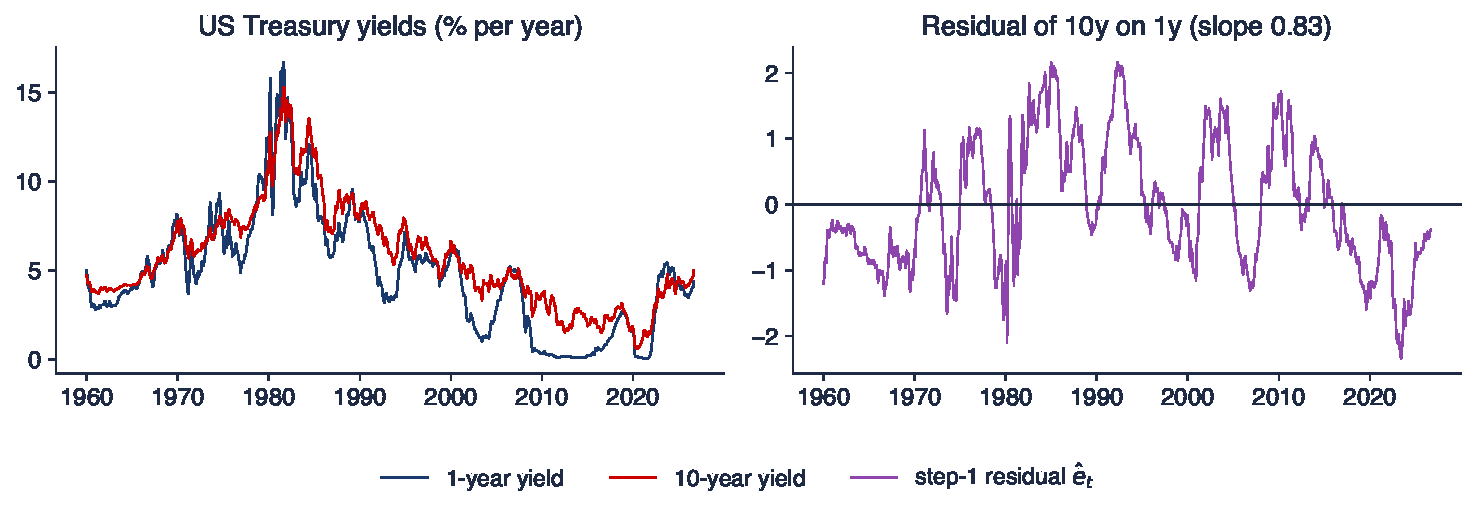
\includegraphics[width=0.96\textwidth,height=0.34\textheight,keepaspectratio]{ch7_sem_b1.pdf}
\end{center}
\vspace{-2mm}
\begin{itemize}
    \item ADF p = 0.26 (1 year), 0.63 (10 years): unit roots; the change: p $<$\,0.001; both yields $I(1)$
    \item Step 1: $\hat\imath^{(10)}_t = 1.76 + 0.827\,i^{(1)}_t$; step 2: $\tau = -3.59$ (19 lags) $< -3.34$: cointegration at 5\% (p = 0.025); Phillips--Ouliaris $Z_t = -3.65$ (p = 0.022)
    \item ECM, 10 years: $\hat\gamma = -0.0295$ ($t = -4.81$), $\hat\delta_0 = 0.53$; 1 year: $\hat\gamma = 0.0172$ ($t = 1.25$), not significant
    \item Interpretation: half-life $\ln 0.5/\ln(1 -0.0295) = 23.1$ months, about two years; the 10-year yield closes the gap, the 1-year yield (set by monetary policy) does not react
\end{itemize}\quantlet{TSA\_ch7\_seminar}{\qlurl{TSA_ch7_seminar}}
\end{frame}

\begin{frame}{B2: consumption and GDP in Romania [Proposed]}
\itemsize{\footnotesize}
\begin{itemize}
\item \textbf{Question}: is Romanian household consumption cointegrated with GDP, as the ``great ratios'' suggest?
\item \textbf{Inputs}: Eurostat, real household consumption and real GDP, chain-linked volumes, seasonally adjusted, 1995--2026; $c_t$, $y_t$ as $100\ln$; model: B1
\item \textbf{Tasks}
\begin{enumerate}
    \item Run ADF (constant and trend) on $c_t$ and $y_t$, and ADF (constant) on their changes.
    \item Run Engle--Granger ($c_t$ on $y_t$) and Phillips--Ouliaris, and report the slope.
    \item Plot the ratio of consumption to GDP and run ADF on $c_t - y_t$.
    \item Interpretation: does a stable consumption share make sense for Romania over 1995--2026?
\end{enumerate}
\item \textbf{Report}: four ADF tests, two cointegration tests, one chart and two sentences
\item Notebook: section B2
\end{itemize}
\end{frame}

\ifsolutions
\begin{frame}{B2: solution [Proposed]}
\itemsize{\scriptsize}
\begin{center}
\includegraphics[width=0.96\textwidth,height=0.34\textheight,keepaspectratio]{ch7_sem_b2.pdf}
\end{center}
\vspace{-2mm}
\begin{itemize}
    \item ADF p = 0.37 ($c_t$), 0.20 ($y_t$); changes: p $<$\,0.001 and $<$\,0.001: both $I(1)$ ($T = 126$)
    \item Slope 1.46; Engle--Granger $\tau = -2.32$ (8 lags), p = 0.36: no cointegration; Phillips--Ouliaris $Z_t = -6.80$, p $<$\,0.001: cointegration; the tests disagree
    \item $c_t - y_t$: ADF p = 0.46; the share rose from about 46\% to 73\% (ratio of chain-linked volumes, a rough measure)
    \item Interpretation: no; a converging economy with growing credit and remittances raised consumption faster than GDP; a slope of 1.46 is not a ``great ratio'', and the verdict depends on the lag choice
\end{itemize}\quantlet{TSA\_ch7\_seminar}{\qlurl{TSA_ch7_seminar}}
\end{frame}
\fi

\begin{frame}{B3: three Central European currencies [Solved]}
\itemsize{\footnotesize}
\begin{itemize}
\item \textbf{Question}: do EUR/RON, EUR/HUF and EUR/PLN share a long-run equilibrium?
\item \textbf{Inputs}: BNR reference rates (cross rates for HUF and PLN), month-end, $100\ln$, since July 2005
\item \textbf{Tasks}
\begin{enumerate}
    \item Run ADF on each rate.
    \item Run the Johansen trace and maximum-eigenvalue tests with a constant and lags by BIC.
    \item Compare with the three pairwise Engle--Granger tests and with the correlations of levels and of changes.
    \item Interpretation: should the three rates be modelled with a VECM?
\end{enumerate}
\item \textbf{Report}: three ADF p-values, a table of six Johansen statistics, a rank and one sentence
\item Notebook: section B3
\end{itemize}
\end{frame}

\begin{frame}{B3: solution [Solved]}
\itemsize{\scriptsize}
\begin{center}
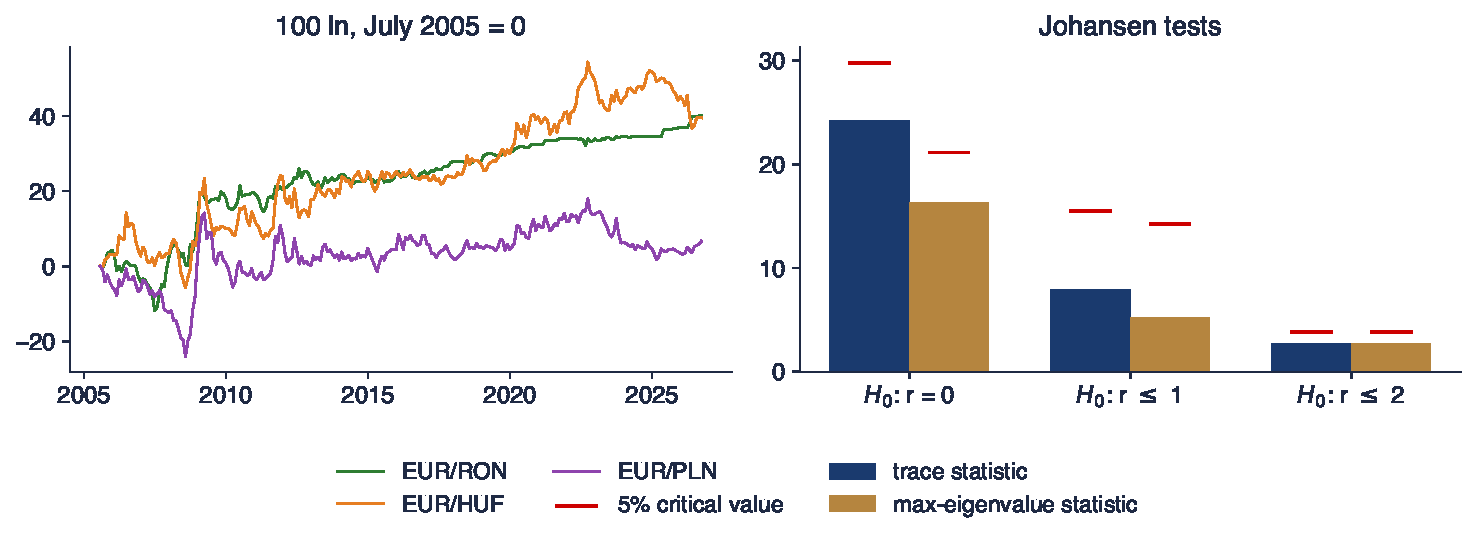
\includegraphics[width=0.96\textwidth,height=0.32\textheight,keepaspectratio]{ch7_sem_b3.pdf}
\end{center}
\vspace{-2mm}
\begin{center}
\scriptsize
\begin{tabular}{lccc}
\toprule
& $r = 0$ & $r \le 1$ & $r \le 2$ \\
\midrule
trace (5\% value) & 24.21 (29.80) & 7.94 (15.49) & 2.72 (3.84) \\
maximum eigenvalue (5\% value) & 16.27 (21.13) & 5.21 (14.26) & 2.72 (3.84) \\
\bottomrule
\end{tabular}
\end{center}
\begin{itemize}
    \item ADF p = 0.55; 0.75; 0.08: three $I(1)$ rates; Johansen ($T = 255$, $k = 1$): no statistic exceeds its critical value: rank 0
    \item Engle--Granger p = 0.29 (RON, HUF), 0.08 (RON, PLN), 0.20 (HUF, PLN); correlation 0.89 in levels but only 0.31 in monthly changes
    \item Interpretation: no; with rank 0 there is no $\beta$ to estimate; model the changes with a VAR in differences (\tsachlink{https://danpele.github.io/Time-Series-Analysis/EN/Courses/chapter6_var_models_granger_causality.pdf}{Chapter 6})
\end{itemize}\quantlet{TSA\_ch7\_seminar}{\qlurl{TSA_ch7_seminar}}
\end{frame}

\begin{frame}{B4: ROBOR, the Romanian 10-year yield and Euribor [Proposed]}
\itemsize{\footnotesize}
\begin{itemize}
\item \textbf{Question}: how many long-run relations tie Romanian interest rates to each other and to Euribor, and which rate adjusts?
\item \textbf{Inputs}: ROBOR 3M and Euribor 3M (Eurostat), Romanian 10-year yield (monthly mean of daily data), January 2010--August 2026; model: B3
\item \textbf{Tasks}
\begin{enumerate}
    \item Run the Johansen tests (constant, BIC lags) and choose the rank.
    \item Estimate the VECM with that rank and the constant restricted to the cointegrating relation; normalise $\beta$ on ROBOR.
    \item Report $\hat\alpha$ with $t$-statistics and run ADF on the equilibrium error.
    \item Interpretation: which rates are weakly exogenous, and what does this say about Romanian monetary conditions?
\end{enumerate}
\item \textbf{Report}: a table of Johansen statistics, $\hat\beta$, $\hat\alpha$ with $t$, one ADF test and two sentences
\item Notebook: section B4
\end{itemize}
\end{frame}

\ifsolutions
\begin{frame}{B4: solution [Proposed]}
\itemsize{\scriptsize}
\begin{center}
\includegraphics[width=0.96\textwidth,height=0.32\textheight,keepaspectratio]{ch7_sem_b4.pdf}
\end{center}
\vspace{-2mm}
\begin{itemize}
    \item $T = 199$, $k = 1$: trace 44.15 $> 29.80$; 14.95 $< 15.49$: rank 1 (the maximum-eigenvalue test agrees)
    \item $\hat\beta^\top\mathbf y_t = \mathrm{ROBOR}_t - 1.38\,i^{(10)}_t + 0.046\,\mathrm{Euribor}_t + 3.67$: ROBOR tied to the Romanian long rate; Euribor almost absent; ADF on the error: p $<$\,0.001
    \item $\hat\alpha$: ROBOR $-0.159$ ($t = -4.72$); 10-year yield $0.024$ ($t = 0.78$); Euribor $-0.005$ ($t = -0.90$)
    \item Interpretation: the 10-year yield and Euribor are weakly exogenous; ROBOR does the adjusting; the long rate reflects inflation and risk premia; Euribor is not the anchor of Romanian money market rates
\end{itemize}\quantlet{TSA\_ch7\_seminar}{\qlurl{TSA_ch7_seminar}}
\end{frame}
\fi


%=============================================================================
\section{Part C: open questions and AI critique}
%=============================================================================

\begin{frame}{C1: pairs trading on two banks [Proposed]}
\itemsize{\footnotesize}
\begin{itemize}
\item \textbf{Question}: would a trader who found Banca Transilvania and BRD cointegrated at the end of 2021 have earned money afterwards?
\item \textbf{Inputs}: adjusted daily prices, formation 2014--2021, trading January 2022--September 2026; models: B1, B3
\item \textbf{Tasks}
\begin{enumerate}
    \item On the formation period, run Engle--Granger and Phillips--Ouliaris (TLV on BRD) and keep $\hat b$, the mean and the standard deviation of the spread.
    \item On the trading period, apply the rule: open at $|z| > 2$, close at $z = 0$; compute the annual return gross and net of 0.20\% per unit traded.
    \item Repeat the Engle--Granger test on the trading period alone.
    \item Interpretation: is the result evidence that pairs trading works on the BVB?
\end{enumerate}
\item \textbf{Report}: two tests, the number of trades, two returns and a plan for a project
\item Notebook: section C1
\end{itemize}
\end{frame}

\ifsolutions
\begin{frame}{C1: reference analysis [Proposed]}
\itemsize{\scriptsize}
\begin{center}
\includegraphics[width=0.96\textwidth,height=0.32\textheight,keepaspectratio]{ch7_sem_c1.pdf}
\end{center}
\vspace{-2mm}
\begin{itemize}
    \item Formation: $\hat b = 1.49$, Engle--Granger p = 0.028, Phillips--Ouliaris p = 0.065: cointegrated at 5\% by one test only
    \item Trading: 3 trades; gross 5.93\% per year (Sharpe 0.68), net 5.67\% (Sharpe 0.66); the spread fell to $z = -4.40$ before it came back
    \item On 2022--2026 alone: Engle--Granger p = 0.12, slope 1.19: the relation weakened; in-sample, full-period parameters: 3.30\% per year
    \item Interpretation: no; 3 trades are an anecdote, one pair was chosen after the fact, and a spread at $z = -4.40$ could also have kept falling; Lecture 7 tests 28 pairs with rolling windows
    \item Project: pairs trading on the BVB with rolling selection, several thresholds, realistic costs and limits on short selling
\end{itemize}\quantlet{TSA\_ch7\_seminar}{\qlurl{TSA_ch7_seminar}}
\end{frame}
\fi

\begin{frame}{C2: audit an AI answer [Proposed]}
\itemsize{\scriptsize}
\begin{itemize}
    \item A student asked an AI assistant about cointegration. The answer:
    \item \aiprompt{(a) The Engle-Granger statistic is -3.0 with two variables; since -3.0 < -2.87, the 5\% Dickey-Fuller value, the series are cointegrated.}
    \item \aiprompt{(b) The ECM coefficient of the lagged equilibrium error is +0.15, so 15\% of the gap is corrected each period.}
    \item \aiprompt{(c) Johansen rejects r = 0 and r <= 1 but not r <= 2 for three yields, so the yields share two common trends.}
    \item \aiprompt{(d) EUR/RON and EUR/HUF are both I(1) and R2 = 0.79 in levels, so they are cointegrated.}
    \item \aiprompt{(e) If two series are cointegrated, at least one of them Granger-causes the other.}
    \item \aiprompt{(f) A pairs-trading rule with a Sharpe ratio of 0.44 on 2014-2026 data will keep this Sharpe ratio in the future.}
    \item Tasks
    \begin{itemize}
        \item 1. For each statement, say whether it is correct; if not, give the correct statement and, where possible, the correct number from the notebook (section C2).
        \item 2. Report: a list of six verdicts with one line of justification each.
    \end{itemize}
\end{itemize}
\end{frame}

\ifsolutions
\begin{frame}{C2: solution [Proposed]}
\itemsize{\scriptsize}
\begin{itemize}
    \item (a) Wrong: residual-based tests need the Engle--Granger value, about $-3.36$; $-3.0 > -3.36$: no cointegration at 5\%
    \item (b) Wrong: a positive coefficient pushes $y$ further from equilibrium; error correction needs a negative coefficient
    \item (c) Wrong: rank 2 means two cointegrating vectors and $3 - 2 = 1$ common trend
    \item (d) Wrong: a high $R^2$ between $I(1)$ series proves nothing; Engle--Granger p = 0.29
    \item (e) Correct: by the Granger representation theorem, at least one adjustment coefficient is non-zero, so the lagged levels help predict at least one variable
    \item (f) Wrong: the 0.44 uses full-sample parameters and a pair chosen after the fact; out of sample the rolling rule earns close to zero after costs (Lecture 7)
\end{itemize}\quantlet{TSA\_ch7\_seminar}{\qlurl{TSA_ch7_seminar}}
\end{frame}
\fi


%=============================================================================
\section{Wrap-up}
%=============================================================================

\begin{frame}{Key takeaways}
\itemsize{\small}
\begin{itemize}
    \item Test that every series is $I(1)$ first; then test the equilibrium error, never the correlation of levels
    \item Residual-based tests need Engle--Granger critical values, which depend on the number of variables
    \item The ECM gives the speed of adjustment; the half-life $\ln 0.5/\ln(1 + \gamma)$ is in the units of the data
    \item Johansen gives the rank; $n - r$ is the number of common trends; $\alpha$ shows who adjusts
    \item An AI answer is a draft: check the critical values, the signs and the number of trends
\end{itemize}
\end{frame}

\begin{frame}{After the seminar}
\itemsize{\small}
\begin{itemize}
    \item Lecture 7 develops each topic of today: common trends, the Engle--Granger distribution, ECM, the VECM and the Granger representation theorem, the Johansen tests, forecasting and pairs trading
    \item Try the [Proposed] tasks in the notebook
    \item C1 can grow into a team project: pairs trading on the BVB, out of sample and after costs
    \item Reading: \refHP, Ch.~9; \refHamilton, Ch.~19--20; \refEG
    \item \textbf{The seminar is for practice and is not graded; the solutions of [Proposed] tasks are discussed in class}
\end{itemize}
\end{frame}


%=============================================================================
\section{References}
%=============================================================================

\begin{frame}{References}
\itemsize{\tiny}
\begin{itemize}
    \item Engle, R. F., \& Granger, C. W. J. (1987). Co-integration and error correction: Representation, estimation, and testing. \textit{Econometrica}, 55(2), 251--276. \href{https://doi.org/10.2307/1913236}{doi:10.2307/1913236}
    \item Gatev, E., Goetzmann, W. N., \& Rouwenhorst, K. G. (2006). Pairs trading: Performance of a relative-value arbitrage rule. \textit{Review of Financial Studies}, 19(3), 797--827. \href{https://doi.org/10.1093/rfs/hhj020}{doi:10.1093/rfs/hhj020}
    \item Hamilton, J. D. (1994). \textit{Time Series Analysis}. Princeton University Press. \href{https://doi.org/10.2307/j.ctv14jx6sm}{doi:10.2307/j.ctv14jx6sm}
    \item Huang, C., \& Petukhina, A. (2022). \textit{Applied Time Series Analysis and Forecasting with Python}. Springer. \href{https://doi.org/10.1007/978-3-031-13584-2}{doi:10.1007/978-3-031-13584-2}
    \item Johansen, S. (1988). Statistical analysis of cointegration vectors. \textit{Journal of Economic Dynamics and Control}, 12(2--3), 231--254. \href{https://doi.org/10.1016/0165-1889(88)90041-3}{doi:10.1016/0165-1889(88)90041-3}
    \item Johansen, S. (1991). Estimation and hypothesis testing of cointegration vectors in Gaussian vector autoregressive models. \textit{Econometrica}, 59(6), 1551--1580. \href{https://doi.org/10.2307/2938278}{doi:10.2307/2938278}
    \item MacKinnon, J. G. (2010). Critical values for cointegration tests. Queen's Economics Department Working Paper No.~1227, Queen's University. \href{https://ideas.repec.org/p/qed/wpaper/1227.html}{ideas.repec.org/p/qed/wpaper/1227}
    \item Phillips, P. C. B., \& Ouliaris, S. (1990). Asymptotic properties of residual based tests for cointegration. \textit{Econometrica}, 58(1), 165--193. \href{https://doi.org/10.2307/2938339}{doi:10.2307/2938339}
\end{itemize}
\end{frame}

\end{document}
